% Options for packages loaded elsewhere
% Options for packages loaded elsewhere
\PassOptionsToPackage{unicode}{hyperref}
\PassOptionsToPackage{hyphens}{url}
\PassOptionsToPackage{dvipsnames,svgnames,x11names}{xcolor}
%
\documentclass[
  12pt,
]{article}
\usepackage{xcolor}
\usepackage[margin=2cm]{geometry}
\usepackage{amsmath,amssymb}
\setcounter{secnumdepth}{5}
\usepackage{iftex}
\ifPDFTeX
  \usepackage[T1]{fontenc}
  \usepackage[utf8]{inputenc}
  \usepackage{textcomp} % provide euro and other symbols
\else % if luatex or xetex
  \usepackage{unicode-math} % this also loads fontspec
  \defaultfontfeatures{Scale=MatchLowercase}
  \defaultfontfeatures[\rmfamily]{Ligatures=TeX,Scale=1}
\fi
\usepackage{lmodern}
\ifPDFTeX\else
  % xetex/luatex font selection
  \setmainfont[]{Times New Roman}
\fi
% Use upquote if available, for straight quotes in verbatim environments
\IfFileExists{upquote.sty}{\usepackage{upquote}}{}
\IfFileExists{microtype.sty}{% use microtype if available
  \usepackage[]{microtype}
  \UseMicrotypeSet[protrusion]{basicmath} % disable protrusion for tt fonts
}{}
\usepackage{setspace}
\makeatletter
\@ifundefined{KOMAClassName}{% if non-KOMA class
  \IfFileExists{parskip.sty}{%
    \usepackage{parskip}
  }{% else
    \setlength{\parindent}{0pt}
    \setlength{\parskip}{6pt plus 2pt minus 1pt}}
}{% if KOMA class
  \KOMAoptions{parskip=half}}
\makeatother
% Make \paragraph and \subparagraph free-standing
\makeatletter
\ifx\paragraph\undefined\else
  \let\oldparagraph\paragraph
  \renewcommand{\paragraph}{
    \@ifstar
      \xxxParagraphStar
      \xxxParagraphNoStar
  }
  \newcommand{\xxxParagraphStar}[1]{\oldparagraph*{#1}\mbox{}}
  \newcommand{\xxxParagraphNoStar}[1]{\oldparagraph{#1}\mbox{}}
\fi
\ifx\subparagraph\undefined\else
  \let\oldsubparagraph\subparagraph
  \renewcommand{\subparagraph}{
    \@ifstar
      \xxxSubParagraphStar
      \xxxSubParagraphNoStar
  }
  \newcommand{\xxxSubParagraphStar}[1]{\oldsubparagraph*{#1}\mbox{}}
  \newcommand{\xxxSubParagraphNoStar}[1]{\oldsubparagraph{#1}\mbox{}}
\fi
\makeatother


\usepackage{longtable,booktabs,array}
\usepackage{calc} % for calculating minipage widths
% Correct order of tables after \paragraph or \subparagraph
\usepackage{etoolbox}
\makeatletter
\patchcmd\longtable{\par}{\if@noskipsec\mbox{}\fi\par}{}{}
\makeatother
% Allow footnotes in longtable head/foot
\IfFileExists{footnotehyper.sty}{\usepackage{footnotehyper}}{\usepackage{footnote}}
\makesavenoteenv{longtable}
\usepackage{graphicx}
\makeatletter
\newsavebox\pandoc@box
\newcommand*\pandocbounded[1]{% scales image to fit in text height/width
  \sbox\pandoc@box{#1}%
  \Gscale@div\@tempa{\textheight}{\dimexpr\ht\pandoc@box+\dp\pandoc@box\relax}%
  \Gscale@div\@tempb{\linewidth}{\wd\pandoc@box}%
  \ifdim\@tempb\p@<\@tempa\p@\let\@tempa\@tempb\fi% select the smaller of both
  \ifdim\@tempa\p@<\p@\scalebox{\@tempa}{\usebox\pandoc@box}%
  \else\usebox{\pandoc@box}%
  \fi%
}
% Set default figure placement to htbp
\def\fps@figure{htbp}
\makeatother


% definitions for citeproc citations
\NewDocumentCommand\citeproctext{}{}
\NewDocumentCommand\citeproc{mm}{%
  \begingroup\def\citeproctext{#2}\cite{#1}\endgroup}
\makeatletter
 % allow citations to break across lines
 \let\@cite@ofmt\@firstofone
 % avoid brackets around text for \cite:
 \def\@biblabel#1{}
 \def\@cite#1#2{{#1\if@tempswa , #2\fi}}
\makeatother
\newlength{\cslhangindent}
\setlength{\cslhangindent}{1.5em}
\newlength{\csllabelwidth}
\setlength{\csllabelwidth}{3em}
\newenvironment{CSLReferences}[2] % #1 hanging-indent, #2 entry-spacing
 {\begin{list}{}{%
  \setlength{\itemindent}{0pt}
  \setlength{\leftmargin}{0pt}
  \setlength{\parsep}{0pt}
  % turn on hanging indent if param 1 is 1
  \ifodd #1
   \setlength{\leftmargin}{\cslhangindent}
   \setlength{\itemindent}{-1\cslhangindent}
  \fi
  % set entry spacing
  \setlength{\itemsep}{#2\baselineskip}}}
 {\end{list}}
\usepackage{calc}
\newcommand{\CSLBlock}[1]{\hfill\break\parbox[t]{\linewidth}{\strut\ignorespaces#1\strut}}
\newcommand{\CSLLeftMargin}[1]{\parbox[t]{\csllabelwidth}{\strut#1\strut}}
\newcommand{\CSLRightInline}[1]{\parbox[t]{\linewidth - \csllabelwidth}{\strut#1\strut}}
\newcommand{\CSLIndent}[1]{\hspace{\cslhangindent}#1}



\setlength{\emergencystretch}{3em} % prevent overfull lines

\providecommand{\tightlist}{%
  \setlength{\itemsep}{0pt}\setlength{\parskip}{0pt}}



 


\usepackage[noblocks]{authblk}
\renewcommand*{\Authsep}{, }
\renewcommand*{\Authand}{, }
\renewcommand*{\Authands}{, }
\renewcommand\Affilfont{\small}
\makeatletter
\@ifpackageloaded{caption}{}{\usepackage{caption}}
\AtBeginDocument{%
\ifdefined\contentsname
  \renewcommand*\contentsname{Table of contents}
\else
  \newcommand\contentsname{Table of contents}
\fi
\ifdefined\listfigurename
  \renewcommand*\listfigurename{List of Figures}
\else
  \newcommand\listfigurename{List of Figures}
\fi
\ifdefined\listtablename
  \renewcommand*\listtablename{List of Tables}
\else
  \newcommand\listtablename{List of Tables}
\fi
\ifdefined\figurename
  \renewcommand*\figurename{Figure}
\else
  \newcommand\figurename{Figure}
\fi
\ifdefined\tablename
  \renewcommand*\tablename{Table}
\else
  \newcommand\tablename{Table}
\fi
}
\@ifpackageloaded{float}{}{\usepackage{float}}
\floatstyle{ruled}
\@ifundefined{c@chapter}{\newfloat{codelisting}{h}{lop}}{\newfloat{codelisting}{h}{lop}[chapter]}
\floatname{codelisting}{Listing}
\newcommand*\listoflistings{\listof{codelisting}{List of Listings}}
\makeatother
\makeatletter
\makeatother
\makeatletter
\@ifpackageloaded{caption}{}{\usepackage{caption}}
\@ifpackageloaded{subcaption}{}{\usepackage{subcaption}}
\makeatother
\usepackage{bookmark}
\IfFileExists{xurl.sty}{\usepackage{xurl}}{} % add URL line breaks if available
\urlstyle{same}
\hypersetup{
  pdftitle={Justification trajectories for pension inequality in Chile (2016-2023): The role of beliefs in meritocracy and social stratification},
  pdfauthor={Juan Carlos Castillo; René Canales; Andreas Laffert; Tomás Urzúa},
  colorlinks=true,
  linkcolor={blue},
  filecolor={Maroon},
  citecolor={Blue},
  urlcolor={Blue},
  pdfcreator={LaTeX via pandoc}}


\title{Justification trajectories for pension inequality in Chile
(2016-2023): The role of beliefs in meritocracy and social
stratification}


  \author{Juan Carlos Castillo}
            \affil{%
                  Departament of Sociology, University of Chile
              }
        \author{René Canales}
            \affil{%
                  Institute of Sociology, Pontifical Catholic University
                  of Chile
              }
        \author{Andreas Laffert}
            \affil{%
                  Institute of Sociology, Pontifical Catholic University
                  of Chile
              }
        \author{Tomás Urzúa}
            \affil{%
                  Departament of Sociology, University of Chile
              }
      
\date{}
\begin{document}
\maketitle
\begin{abstract}
My abstract \newline \textbf{Keywords}: Economic inequality,
meritocracy, market justice, Chile, public preferences
\end{abstract}


\setstretch{1.15}
\section{Introduction}\label{introduction}

The pension system is at the core of the welfare state, playing a key
role in shaping income distribution among the elderly population
(\citeproc{ref-breznau_institutional_2023}{Breznau, 2023};
\citeproc{ref-esping-andersen_three_1990}{Esping-Andersen, 1990}). This
system is based on a shared understanding that older adults require
financial support after retirement, whereby pensions are designed to
provide such support. In such an understanding, justice principles held
in a society are crucial, as they influence how individuals perceive the
fairness of pension systems and the distribution of benefits in a
society (\citeproc{ref-liebig_sociology_2016}{Liebig \& Sauer, 2016}).
For instance, in systems that emphasize social solidarity, there may be
a greater support towards redistributive mechanisms to ensure a more
equitable distribution of pension benefits across different social
groups. Conversely, in societies where meritocratic beliefs are
prevalent, individuals may justify inequalities in pension benefits
based on factors such as work history, contributions to the system, and
individual effort (\citeproc{ref-castillo_socialization_2024}{Juan
Carlos Castillo et al., 2024}; \citeproc{ref-mijs_paradox_2019}{Mijs,
2019}).

The Chilean pension system is a classical case study when it comes to
privatization based on individual contributions, whereby those with
higher lifetime earnings tend to receive higher pension benefits, while
those with lower earnings often face inadequate pensions. Such system
has created large disparities and increased poverty rates among the
elderly, making them struggle to make ends meet
(\citeproc{ref-borzutzky_chiles_2016}{Borzutzky \& Hyde, 2016};
\citeproc{ref-bril-mascarenhas_how_2019}{Bril-Mascarenhas \& Maillet,
2019}; \citeproc{ref-cabib_avoiding_2025}{Cabib, 2025};
\citeproc{ref-evans_assessing_2024}{C. Evans \& Pienknagura, 2024};
\citeproc{ref-subsecretariadeprevisionsocial_percepcion_2023}{Subsecretaría
de Previsión Social, 2023}). In this scenario, a deep discontent and
social movements demanding reforms of the pension system have emerged in
recent years. Nevertheless, and despite this discontent, some studies
have shown that an important and growing share of the population is
willing to justify inequalities in pensions based on individual
contributions (\citeproc{ref-castillo_perceptions_2025}{Juan Carlos
Castillo et al., 2025}). In such a context, understanding how
meritocratic beliefs and social class influence the justification of
inequalities in pensions acquires relevance for informing policy debates
and promoting social justice
(\citeproc{ref-busemeyer_welfare_2020}{Busemeyer \& Iversen, 2020};
\citeproc{ref-svallfors_moral_2006}{Svallfors, 2006}).

The concept of market justice refers to the belief that the distribution
of goods and services (as pensions) should be determined by market
mechanisms, such as supply and demand, rather than by social or
political considerations (\citeproc{ref-lane_market_1986}{Lane, 1986};
\citeproc{ref-lindh_public_2015}{Lindh, 2015}). More specifically,
research on market justice focuses on individual payment capacity and
contribution as the main criteria for distributing resources,
emphasizing personal responsibility and effort over collective welfare
(\citeproc{ref-castillo_socialization_2024}{Juan Carlos Castillo et al.,
2024};
\citeproc{ref-wilson_market_1997}{\textbf{wilson\_market\_1997?}}).
Within this framework, the present paper aims to analyze how
meritocratic beliefs and social class are associated with the
preferences of market justice in pensions in Chile, and how these
associations have evolved between 2016 and 2023. On the one hand, social
class has been shown to influence individuals' perceptions of justice
and fairness in various social contexts, including pensions, as it
shapes their experiences and access to resources
(\citeproc{ref-svallfors_moral_2006}{Svallfors, 2006}). In this regard,
individuals from higher social classes may be more likely to justify
inequalities in pensions, as they may benefit more from the existing
system. On the other hand, meritocracy is a widely held belief that
individuals should be rewarded based on their abilities and efforts
(\citeproc{ref-mcnamee_meritocracy_2004}{McNamee \& Miller, 2004};
\citeproc{ref-young_rise_1975}{Young, 1975}). In the context of
pensions, this belief may lead individuals to justify inequalities in
pension benefits based on their contributions to the system.

To address these issues, we utilize data from the Chilean Longitudinal
Social Survey (ELSOC) conducted between 2016 and 2023. This survey
provides a comprehensive overview of public attitudes towards social
justice issues in Chile, including perceptions of pensions and income
distribution. By analyzing this data, we aim to shed light on the
complex interplay between meritocratic beliefs, social class, and the
justification of inequalities in pensions in Chile over time.

The paper is structured as follows. First, we review the relevant
literature on meritocratic beliefs, social class, and the justification
of inequalities in pensions. Next, we describe the data and methodology
used in our analysis. We then present our findings on the associations
between meritocratic beliefs, social class, and the justification of
inequalities in pensions in Chile from 2016 to 2023. Finally, we discuss
the implications of our findings for policy and future research.

\section{Market justice}\label{market-justice}

In recent years, welfare states have undergone several institutional
transformations, with market expansion strongly penetrating the field of
social services and rights, while private alternatives emerge in
parallel to public provision
(\citeproc{ref-busemeyer_welfare_2020}{Busemeyer \& Iversen, 2020}).
Such processes have led to changes in the architecture of the
institutions responsible for social welfare, where private companies
operate as service administrators that limit access based on the user's
ability to pay, while public providers have reorganized to compete as
quasi-markets (\citeproc{ref-lindh_it_2017}{Lindh, 2017}). Despite the
commodification of services, this does not only imply changes at the
formal level, but also shapes the beliefs of individuals. In this way,
market-oriented policies can modify people's normative criteria,
promoting or weakening support for different goods or services. This
phenomenon is known as \emph{policy feedback
effect}.(\citeproc{ref-beland_varieties_2019}{Béland \& Schlager, 2019};
\citeproc{ref-jaime-castillo_public_2013}{Jaime-Castillo, 2013}).

In distributive justice field, market preferences have gained relevance
in attitudinal studies on redistribution. In this context, market
justice emerges as one of the central concepts in this literature,
understood as a normative principle that legitimizes access to goods and
services based on individual or family ability to pay, the basis of
which is radically opposed to social justice
(\citeproc{ref-lane_market_1986}{Lane, 1986}). This market-oriented
redistribution is closely related to the justification of inequalities,
as it considers the market to be a space of equal opportunity, where
economic success is understood as an individual outcome
(\citeproc{ref-kluegel_legitimation_1999}{J. Kluegel et al., 1999}). In
this way, market justice legitimizes socioeconomic inequalities from an
economic-moral perspective, ignoring the structural conditions that
generate disparities.

Research strategies on market preferences have focused on
operationalizing this concept in order to empirically study how
individuals' beliefs are shaped by macro-structural conditions, such as
the application of privatization policies to goods such as education,
health, or pensions (\citeproc{ref-busemeyer_education_2013}{Busemeyer,
2013}; \citeproc{ref-kerner_pension_2020}{Kerner, 2020};
\citeproc{ref-lindh_public_2015}{Lindh, 2015}). The inaugural study in
this line of research was by J. R. Kluegel \& Smith
(\citeproc{ref-kluegel_beliefs_1981}{1981}), analyzing the normative
bases of beliefs about social stratification. Subsequently, market
preferences have been studied in detail in surveys, where International
Social Survey Program (ISSP) has led the comparative study between
countries focused on social inequality, asking how fair it is considered
that those with higher incomes have access to better education, health,
and/or pensions from 1999 to the present day
(\citeproc{ref-immergut_it_2020}{Immergut \& Schneider, 2020};
\citeproc{ref-lindh_public_2015}{Lindh, 2015}). In this frame, ISSP has
been one of the most important resources for building a market justice
agenda. There are also studies that have measured market preferences
using an index constructed from three items referring to market justice
in the three main social services, operationalizing the concept of
preferences for market justice
(\citeproc{ref-castillo_perceptions_2025}{Juan Carlos Castillo et al.,
2025}). In short, all the strategies employed seek to understand the
extent to which market-generated inequalities are legitimized.

Recent literature on market preferences has found striking associations
with both individual and contextual factors. Various studies suggest
that people with higher socioeconomic status tend to adopt greater
market preferences than those who are in a more disadvantaged social
position (\citeproc{ref-koos_moral_2019}{Koos \& Sachweh, 2019};
\citeproc{ref-lindh_public_2015}{Lindh, 2015}). Similarly, political
ideology has been linked to preferences for market justice, with
right-wing individuals mostly supporting market-oriented distribution
(\citeproc{ref-castillo_socialization_2024}{Juan Carlos Castillo et al.,
2024}; \citeproc{ref-lee_fairness_2024}{Lee \& Stacey, 2024}). These
trends reflect a moral economy based on the justification of status by
those who enjoy the benefits of the market. With regard to contextual
factors, evidence suggests that in countries with greater private
investment in services, individuals tend to decrease their preferences
for redistribution, internalizing the market order as a criterion of
justice, while in countries where public provision of services prevails,
individuals show resistance to market-induced inequalities
(\citeproc{ref-busemeyer_education_2013}{Busemeyer, 2013};
\citeproc{ref-immergut_it_2020}{Immergut \& Schneider, 2020};
\citeproc{ref-lindh_public_2015}{Lindh, 2015}).

In the market justice frame, pensions have been one of the most studied
elements due to their centrality in discussions of economic distribution
among the elderly population
(\citeproc{ref-arenas_sistemas_2019}{Arenas, 2019}). Some pension
systems are based on principles of solidarity, demonstrating solid
security systems. On the other hand, there are pension systems based on
privatization policies, managing resources according to market logic
such as investments, which runs counter to principles of solidarity
(\citeproc{ref-arrizabalomontoro_debate_2019}{Arrizabalo Montoro et al.,
2019}). Pension system policies have cultural implications for
societies. For example, market-oriented plans are associated with
feelings of insecurity due to the individualization of risk.
(\citeproc{ref-yen_pension_2018}{\textbf{yen\_pension\_2018?}}). From a
broader perspective, depending on the policies applied in pension
systems, these have a positive or negative effect on preferences for
market justice (\citeproc{ref-castillo_perceptions_2025}{Juan Carlos
Castillo et al., 2025}).

\section{Meritocracy}\label{meritocracy}

Meritocracy is a normative principle that justifies the distribution of
goods and services based on individual effort and talent, emphasizing
that rewards should correspond to personal achievements rather than
social status or inherited privileges
(\citeproc{ref-young_rise_1958}{\textbf{young\_rise\_1958?}};
\citeproc{ref-sandel_tyranny_2020}{\textbf{sandel\_tyranny\_2020?}}).
This concept has gained prominence in contemporary societies, where
meritocratic ideals are often invoked to legitimize socioeconomic
inequalities, suggesting that individuals' success or failure is
primarily determined by their own merits
(\citeproc{ref-littler_meritocracy_2018}{Littler, 2018}).

Research on meritocratic beliefs has explored how individuals perceive
the fairness of social systems that prioritize merit-based distribution.
Studies have shown that people who strongly endorse meritocratic ideals
tend to justify existing inequalities, attributing success to personal
effort and downplaying the role of structural factors such as social
class (\citeproc{ref-reynolds_perceptions_2014}{Reynolds \& Xian,
2014}). This perspective can lead to reduced support for redistributive
policies, as individuals may view such interventions as undermining the
principles of meritocracy (\citeproc{ref-piketty_capital_2014}{Piketty,
2014}).

Empirical investigations have also examined the relationship between
meritocratic beliefs and various demographic and ideological factors.
For instance, individuals with higher socioeconomic status are more
likely to endorse meritocratic ideals, as they often benefit from
systems that reward their efforts and talents
(\citeproc{ref-harrs_fairness_2025}{Harrs \& Sterba, 2025}).
Additionally, political ideology plays a significant role, with
right-leaning individuals typically exhibiting stronger support for
meritocracy compared to their left-leaning counterparts. Contextual
factors also influence meritocratic beliefs. Although in in societies
with high levels of social mobility and equal opportunities, individuals
may be more inclined to endorse meritocratic ideals, some evidence
suggest that ienquality is linked to larger meritocratic perception, aka
the paradox of meritocracy (\citeproc{ref-mijs_paradox_2021}{Mijs,
2021}). Overall, the concept of meritocracy remains a central theme in
discussions about social justice and inequality, highlighting the
complex interplay between individual effort, structural conditions, and
societal values.

The measurement of meritocratic beliefs has been approached through
various survey instruments that assess individuals' attitudes towards
effort, talent, and the fairness of merit-based systems. Commonly used
items include questions about the importance of hard work for success,
the role of innate ability, and perceptions of fairness in competitive
environments (\citeproc{ref-castillo_multidimensional_2023}{Juan Carlos
Castillo et al., 2023}). In the extant literature the measurement of
meritocratic beliefs has often been inconsistent, with different studies
employing varying scales and items, making cross-study comparisons
challenging. To address this issue, some researchers have advocated for
the development of standardized measures that capture the multifaceted
nature of meritocratic beliefs. A first distiction to make here is the
one between perceptions and preferences for meritocracy, usually the
first being descriptive and the second more normative in nature
(\citeproc{ref-castillo_multidimensional_2023}{Juan Carlos Castillo et
al., 2023}). Research on meritocratic perceptions have reveal that
people's beliefs about the extent to which meritocracy exists in society
can differ significantly from their normative support for meritocratic
principles (\citeproc{ref-castillo_multidimensional_2023}{Juan Carlos
Castillo et al., 2023}). Besides, whereas meritocratic preferences are
usually more consensual, meritocratic perceptions tend to vary more
across individuals and contexts.

\section{Class}\label{class}

Despite criticism of class analysis as a category for studying social
order (\citeproc{ref-pakulski_death_1997}{Pakulski \& Waters, 1997}),
various contemporary studies have shown that class inequalities remain
relevant as a subject of research for explaining attitudes towards
social justice (\citeproc{ref-dodson_economic_2017}{Dodson, 2017};
\citeproc{ref-lindh_public_2015a}{\textbf{lindh\_public\_2015a?}};
\citeproc{ref-lindh_class_2020a}{\textbf{lindh\_class\_2020a?}}).
Different approaches, from neo-Marxist
(\citeproc{ref-wright_class_2000}{Wright, 2000}) to neo-Weberian
(\citeproc{ref-breen_foundations_2005}{Breen, 2005}), agree that
people's different socioeconomic positions act as determinants of how
material interests and shared life experiences structure individuals'
subjective perceptions of social reality and the justification of
certain inequalities present in the system
(\citeproc{ref-bottero_class_2004a}{\textbf{bottero\_class\_2004a?}}).

Material interests derived from class position constitute a fundamental
bridge between the objective structure of inequality, perceptions of
justice, political positioning, and distribution of resources
(\citeproc{ref-evans_conditional_2022}{G. Evans et al., 2022};
\citeproc{ref-langsaether_more_2020}{Langsæther \& Evans, 2020};
\citeproc{ref-bottero_class_2004a}{\textbf{bottero\_class\_2004a?}}).
Along these lines, various studies recognise that the position
individuals occupy in the class structure---whether subordinate or
privileged---produces significant variations in how they perceive and
justify different social inequalities within market frameworks
(\citeproc{ref-langsaether_more_2020}{Langsæther \& Evans, 2020};
\citeproc{ref-svallfors_moral_2006}{Svallfors, 2006}). In the context of
pension systems based on individual contributions, such as the Chilean
system, these distinctions are particularly relevant, as they allow us
to differentiate preferences and perceptions regarding a system from
which some people benefit while others remain in vulnerable positions
according to their class position.

Class theory in welfare states suggests that positions in the labour
market define similarities in economic resources, opportunities and
constraints, structuring both economic interests and group identities
(\citeproc{ref-erikson_constant_1992}{Erikson \& Goldthorpe, 1992a};
\citeproc{ref-korpi_new_2003}{Korpi \& Palme, 2003}). From this
perspective, the strong dependence on market linkages in distributive
processes mainly empowers class categories that are well equipped with
scarce productive resources, while people in positions characterised by
fewer marketable resources benefit more from political distribution
based on social citizenship (\citeproc{ref-korpi_power_2006}{Korpi,
2006}, \citeproc{ref-korpi_democratic_2018}{2018}). In the specific case
of social services, different methods of provision have different class
distribution profiles: private financing imposes higher costs on the
individual and links access to the recipient's income profile,
potentially restricting access for low-income or high-risk groups
(\citeproc{ref-gingrich_making_2011}{Gingrich, 2011}). Therefore, from a
rational actor perspective, people in class positions with greater
marketable assets are expected to be more favourable towards market
distribution than those in positions characterised by fewer assets and
greater risks
(\citeproc{ref-lindh_public_2015a}{\textbf{lindh\_public\_2015a?}}).

However, policy feedback theories emphasise that social policy
institutions structure both economic incentives and normative frames of
reference (\citeproc{ref-pierson_when_1993}{Pierson, 1993};
\citeproc{ref-rothstein_just_1998}{Rothstein, 1998};
\citeproc{ref-svallfors_political_2007}{Svallfors, 2007}). This
perspective suggests that class conflict is shaped by institutions, and
that normative beliefs about the market may be influenced by the social
and institutional context in which citizens are embedded
(\citeproc{ref-svallfors_moral_2006}{Svallfors, 2006}). Empirical
research on the relationship between social position and perceptions of
justice has shown a consistent pattern: perceptions of fairness tend to
be structured according to people's social position
(\citeproc{ref-edlund_democratic_2015}{Edlund \& Lindh, 2015};
\citeproc{ref-perezahumada_class_2024}{Pérez Ahumada, 2024}). In this
sense, while the lower classes tend to be less accepting of inequality
and more in favour of redistribution, the upper classes tend to be more
accepting of these inequalities on the basis of meritocratic criteria
(\citeproc{ref-castillo_perceptions_2025}{Juan Carlos Castillo et al.,
2025};
\citeproc{ref-lindh_public_2015a}{\textbf{lindh\_public\_2015a?}};
\citeproc{ref-lindh_class_2020a}{\textbf{lindh\_class\_2020a?}}). This
pattern can be explained by the fact that people in privileged positions
experience less impairment of their material interests and tend to
perceive their own situation as the result of their effort and
qualifications
(\citeproc{ref-lindh_class_2020a}{\textbf{lindh\_class\_2020a?}}), while
justifying access to certain services as fair competition in the market
based on their ability to pay
(\citeproc{ref-castillo_perceptions_2025}{Juan Carlos Castillo et al.,
2025}).

In the specific case of Chile, the individually funded pension system
has generated enormous disparities and vulnerability among the elderly
population, creating a scenario in which the justification for these
inequalities takes on special importance
(\citeproc{ref-borzutzky_chiles_2016}{Borzutzky \& Hyde, 2016};
\citeproc{ref-bril-mascarenhas_how_2019}{Bril-Mascarenhas \& Maillet,
2019}; \citeproc{ref-cabib_avoiding_2025}{Cabib, 2025};
\citeproc{ref-evans_assessing_2024}{C. Evans \& Pienknagura, 2024};
\citeproc{ref-subsecretariadeprevisionsocial_percepcion_2023}{Subsecretaría
de Previsión Social, 2023}). Despite documented social discontent,
recent studies have identified that a significant proportion of the
population is willing to justify pension inequalities based on
meritocratic beliefs and notions of market justice
(\citeproc{ref-castillo_perceptions_2025}{Juan Carlos Castillo et al.,
2025}). This apparent contradiction suggests that beliefs about how
pensions should be distributed do not necessarily align with the
objective material interests of the classes, raising questions about how
social class and meritocratic beliefs interact in the justification of
inequalities.

Understanding how meritocratic beliefs and social position are related
to the justification of pension inequalities is fundamental to
understanding both the persistence of social discontent and the
acceptance of highly unequal systems
(\citeproc{ref-busemeyer_welfare_2020}{Busemeyer \& Iversen, 2020};
\citeproc{ref-svallfors_moral_2006}{Svallfors, 2006}). Preferences for
market justice in pensions represent a specific political expression of
how individuals, based on their class position, evaluate the legitimacy
of a system that distributes resources in a differentiated manner
(\citeproc{ref-iturra-sanhueza_classbased_2025}{Iturra-Sanhueza, 2025}).
However, policy feedback theories suggest that welfare state
institutions not only structure material incentives, but also the
normative frameworks that citizens use to evaluate policy performance
(\citeproc{ref-kerner_pension_2020}{Kerner, 2020};
\citeproc{ref-pierson_when_1993}{Pierson, 1993}). In individually funded
pension systems, investment returns can serve as particularly clear
signals of system performance, influencing how participants
retrospectively judge its effectiveness
(\citeproc{ref-kerner_pension_2020}{Kerner, 2020}). This suggests that
attitudes towards market fairness in pensions are not formed solely on
the basis of static class interests, but also in response to the
perceived performance of the system. Analysing these associations over
time allows us to identify how these justifications evolve and what
factors explain why some groups maintain or modify their assessments of
what constitutes a fair pension system.

\section{Pensions}\label{pensions}

Pension systems occupy a central place in the welfare state, as they
shape the distribution of income and risks in old age
(\citeproc{ref-arenas_sistemas_2019}{Arenas, 2019};
\citeproc{ref-breznau_institutional_2023}{Breznau, 2023};
\citeproc{ref-esping-andersen_three_1990}{Esping-Andersen, 1990}). While
they share the fundamental premise that older adults require financial
support after retirement and that pension income can be understood as
deferred wages reflecting past contributions, the principles of justice
underpinning their design vary considerably across societies
(\citeproc{ref-verbic_political_2019}{Verbič \& Spruk, 2019}). In
contexts where ideals of social solidarity are prominent, redistributive
mechanisms permit a more equal sharing of resources and risks across
social groups. By contrast, where meritocratic beliefs are stronger,
inequalities in pensions are more readily justified in terms of
employment histories, individual contributions, and personal effort
(\citeproc{ref-busemeyer_welfare_2020}{Busemeyer \& Iversen, 2020};
\citeproc{ref-castillo_socialization_2024}{Juan Carlos Castillo et al.,
2024};
\citeproc{ref-mijs_paradox_2019a}{\textbf{mijs\_paradox\_2019a?}};
\citeproc{ref-lindh_public_2015a}{\textbf{lindh\_public\_2015a?}}).
Analysing these justice principles---and their influence on support for
different pension arrangements---is therefore crucial for understanding
the legitimacy of welfare institutions
(\citeproc{ref-mau_inequality_2015}{Mau, 2015}).

Despite sustained economic growth during the 1990s, Chile remains one of
the most unequal countries in Latin America and the OECD
(\citeproc{ref-flores_top_2020}{Flores et al., 2020}). The poorest 50\%
of the population earn around 10\% of total income and hold negative net
wealth, while the wealthiest 1\% receive almost 27\% of income and
control roughly half of national wealth
(\citeproc{ref-chancel_world_2022}{Chancel et al., 2022}). These
inequalities are not simply the outcome of market forces. They are
rooted in neoliberal reforms that privatised and commodified key spheres
of social reproduction (\citeproc{ref-ferre_welfare_2023}{Ferre, 2023};
\citeproc{ref-pnud_desiguales_2017}{PNUD, 2017}). Introduced under the
military dictatorship (1973--1989) and subsequently expanded by
democratic governments, these reforms entrenched market logics in
essential public services through concessions and regulatory frameworks
that favoured private provision, producing a model of commodified public
services that underpins Chile's neoliberal order
(\citeproc{ref-madariaga_three_2020}{Madariaga, 2020}). Health and
education have been extensively studied in this regard
(\citeproc{ref-llambias-wolff_political_2019}{Llambías-Wolff, 2019};
\citeproc{ref-rosenzvaig-hernandez_unmaking_2024}{Rosenzvaig-Hernandez,
2024}), revealing structurally segmented systems in which access and
quality depend heavily on the ability to pay
(\citeproc{ref-castillo_perceptions_2025}{Juan Carlos Castillo et al.,
2025}). In this setting, class trajectories unfold under conditions of
high inequality and market-based provision in core welfare domains,
including pensions.

Since 1981, old-age income security in Chile has been organised
primarily through a fully privatised, mandatory defined-contribution
scheme. A far-reaching reform replaced the previous earnings-related,
pay-as-you-go social insurance system with individual capitalisation
accounts administered by private Pension Fund Administrators (AFP)
(\citeproc{ref-huber_political_2000}{Huber \& Stephens, 2000};
\citeproc{ref-solimano_rise_2021}{Solimano, 2021}). Under this design,
dependent employees must contribute 10\% of their wages, plus an
administrative fee, to individual accounts, while employers face no
mandatory contributions. AFPs invest these savings in domestic and
international financial markets, and since the early 2000s, affiliates
are assigned to, or choose among, several ``multifunds'' (A--E) with
distinct risk--return profiles (\citeproc{ref-hyde_chiles_2015}{Hyde \&
Borzutzky, 2015};
\citeproc{ref-barriga_pensiones_2024}{\textbf{barriga\_pensiones\_2024?}}).
After more than four decades, benefit levels remain modest: for most
retirees, AFP-financed pensions fall below the statutory minimum wage,
and self-funded replacement rates hover around 30\%, even among workers
with long and dense contribution records
(\citeproc{ref-galvez_pensiones_2024}{Gálvez et al., 2024};
\citeproc{ref-madero-cabib_private_2019}{Madero-Cabib et al., 2019}). To
secure a minimum income in old age, the state has progressively
introduced tax-financed solidarity components---most notably the
\emph{Nuevo Pilar Solidario} (2008) and the \emph{Pensión Garantizada
Universal} (PGU, 2022)---which top up low or non-existent contributory
pensions among poorer and lower-middle older adults
(\citeproc{ref-boccardo_30_2020}{Boccardo, 2020}). In practice, this has
produced a hybrid arrangement in which privately managed individual
accounts are substantially subsidised by the state, and tax-funded
transfers constitute a significant share of total pension income at the
bottom of the distribution (\citeproc{ref-galvez_pensiones_2024}{Gálvez
et al., 2024}). For instance, in 2023, half of all old-age pensioners
received less than about the 75\% of the minimum wage, and this figure
drops when state transfers from the PGU or the Solidarity Pension
Contribution are excluded.

This institutional configuration both reflects and reinforces Chile's
broader pattern of persistent inequality combined with extensive welfare
privatisation. Stratified access to social protection has eroded
expectations of upward mobility and contributed to social unrest, with
pensions becoming a focal point of public discontent and protest
(\citeproc{ref-pnud_desiguales_2017}{PNUD, 2017};
\citeproc{ref-rozasbugueno_entre_2019}{Rozas Bugueño \& Maillet, 2019}).
At the same time, the attitudinal landscape is not univocal. Recent
evidence shows that, alongside widespread criticism of the private
pension system and repeated demands for reform, an increasing share of
the population considers pension inequalities based on individual
contribution histories to be fair or legitimate
(\citeproc{ref-castillo_perceptions_2025}{Juan Carlos Castillo et al.,
2025}). These developments are embedded in broader transformations of
Chile's class structure and moral orientations. Meritocratic beliefs
have intensified, accompanying the diffusion of market-centred moral
frameworks in which individuals and families are expected to act as
self-responsible agents, investing in their own ``market value'' and
bearing the risks of their life-course trajectories
(\citeproc{ref-canalesceron_sujeto_2021}{Canales Cerón et al., 2021};
\citeproc{ref-mau_inequality_2015}{Mau, 2015}). In a context marked by
high and durable inequalities, deep marketisation of welfare, and the
growing entrenchment of meritocratic beliefs, it becomes crucial to
examine how pension inequalities are justified, how these justifications
vary across social classes and meritocratic orientations, and how they
have evolved (\citeproc{ref-castillo_perceptions_2025}{Juan Carlos
Castillo et al., 2025}; \citeproc{ref-castillo_socialization_2024}{Juan
Carlos Castillo et al., 2024}).

\subsection{This study}\label{this-study}

First, findings from previous research have found that higher class
position is associated with skepticism toward redistributive policies
(\citeproc{ref-koos_moral_2019}{Koos \& Sachweh, 2019}). More
specifically, the upper classes tend to prefer market-based distribution
to a greater extent than those in less privileged positions
(\citeproc{ref-lindh_public_2015}{Lindh, 2015}). When individuals have
the ability to pay for quality services, their principles of justice
align with this logic, making them more likely to view market mechanisms
as legitimate and accept that the distribution of goods depends on
purchasing power.

Secondly, the literature has pointed out that perceived meritocracy is
positively associated with market preferences for goods and services,
especially pensions, both at a specific point in time and longitudinally
(\citeproc{ref-castillo_perceptions_2025}{Juan Carlos Castillo et al.,
2025}; \citeproc{ref-castillo_deserving_2019}{Juan-Carlos Castillo et
al., 2019}). Those who believe that effort and talent determine success
tend to support market-oriented distribution, as they consider that this
reflects the results of individual effort
(\citeproc{ref-castillo_socialization_2024}{Juan Carlos Castillo et al.,
2024}). In this way, meritocratic perceptions operate as an argument to
legitimize market justice insofar as an individual's ability to pay is
proportional to the effort they have put in.

Additionally, this research examines the interaction between class and
meritocracy in shapingmarket preferences. Specifically, we argue that
the relationship between an individual's socioeconomic position and
market preference for pensions is moderated by meritocratic perceptions.
When individuals have high meritocratic perceptions, the positive
association between class and market preferences for pensions will be
stronger in upper classes than in lower classes. This interaction is
studied at an inter-individual level, and with an exploratory intent, we
also look at how changes over time can reveal an intra-individual
evolution in the way class and meritocracy shape market preferences for
pensions.

Based on the arguments outlined above, we propose the following
hypotheses:

\(H1 \; (\text{Between-person}):\) Those belonging to the upper classes
show, on average, greater support for the commodification of pensions
than those belonging to the lower classes.

\(H2_{a} \; (\text{Between-person}):\) People who perceive more
meritocracy tend to show greater support for the commodification of
pensions than those who hold these perceptions less strongly.

\(H2_{b} \; (\text{Within-person}):\) When the same person strengthens
their meritocratic perceptions over time, their support for the
commodification of pensions increases.

\(H3_{a} \; (\text{Between-person}):\) The positive association between
meritocracy (BE) and support for commodification is stronger in upper
classes.

\(H3_{b} \; (\text{Within-person}):\) When upper-class individuals
increase their meritocratic perceptions over time (WE), their support
for commodification rises more than in lower classes.

\section{Libraries}\label{libraries}

\section{Data, Variables and Methods}\label{data-variables-and-methods}

\subsection{Data}\label{data}

For this study, we used the Chilean Longitudinal Social Survey (ELSOC).
This is a panel study conducted annually between 2016 and 2023, designed
to examine the attitudes, emotions, and behaviours of people aged 18 to
75 with regard to issues of social cohesion and conflict. In terms of
methodology, the survey uses a probabilistic, stratified, clustered,
multistage sampling design covering urban centres and small towns. The
sampling frame is stratified proportionally into six categories of urban
population size, followed by random selection of households within 1,067
blocks.

The survey has been conducted annually since 2016, with the exception of
2020, when it was suspended due to the COVID-19 pandemic. For the
purposes of this study, the 2016, 2017, 2018, 2019, 2022, and 2023 waves
were used. The 2021 wave was excluded because the version of the
questionnaire omitted variables of interest. Between waves 1 and 6,
panel attrition reached 40\%, so a balanced panel was used, resulting in
a final two-level sample comprising \emph{N} = 5,755 observations nested
in \emph{N} = 1,027 individuals. Further details on sampling, attrition,
and weighting procedures are available at
https://coes.cl/encuesta-panel/, and the dataset is publicly accessible
at https://dataverse.harvard.edu/dataverse/elsoc.

\subsection{Variables}\label{variables}

\begin{longtable}[]{@{}
  >{\centering\arraybackslash}p{(\linewidth - 14\tabcolsep) * \real{0.1250}}
  >{\raggedright\arraybackslash}p{(\linewidth - 14\tabcolsep) * \real{0.1250}}
  >{\raggedright\arraybackslash}p{(\linewidth - 14\tabcolsep) * \real{0.1250}}
  >{\raggedright\arraybackslash}p{(\linewidth - 14\tabcolsep) * \real{0.1250}}
  >{\raggedright\arraybackslash}p{(\linewidth - 14\tabcolsep) * \real{0.1250}}
  >{\raggedright\arraybackslash}p{(\linewidth - 14\tabcolsep) * \real{0.1250}}
  >{\centering\arraybackslash}p{(\linewidth - 14\tabcolsep) * \real{0.1250}}
  >{\centering\arraybackslash}p{(\linewidth - 14\tabcolsep) * \real{0.1250}}@{}}

\caption{\label{tbl-summary2}Estadísticos descriptivos variables}

\tabularnewline

\toprule\noalign{}
\begin{minipage}[b]{\linewidth}\centering
\textbf{No}
\end{minipage} & \begin{minipage}[b]{\linewidth}\centering
\textbf{Variable}
\end{minipage} & \begin{minipage}[b]{\linewidth}\centering
\textbf{Label}
\end{minipage} & \begin{minipage}[b]{\linewidth}\centering
\textbf{Stats / Values}
\end{minipage} & \begin{minipage}[b]{\linewidth}\centering
\textbf{Freqs (\% of Valid)}
\end{minipage} & \begin{minipage}[b]{\linewidth}\centering
\textbf{Graph}
\end{minipage} & \begin{minipage}[b]{\linewidth}\centering
\textbf{Valid}
\end{minipage} & \begin{minipage}[b]{\linewidth}\centering
\textbf{Missing}
\end{minipage} \\
\midrule\noalign{}
\endhead
\bottomrule\noalign{}
\endlastfoot
1 & just\_pension {[}factor{]} & Pension distributive justice &
\begin{minipage}[t]{\linewidth}\raggedright
\begin{longtable*}[]{@{}l@{}}
\toprule\noalign{}
\endhead
\bottomrule\noalign{}
\endlastfoot
1. Strongly disagree \\
2. Disagree \\
3. Neither agree nor disagre \\
4. Agree \\
5. Strongly agree \\
\end{longtable}
\end{minipage} & \begin{minipage}[t]{\linewidth}\raggedright
\begin{longtable}[]{@{}rlrl@{}}
\toprule\noalign{}
\endhead
\bottomrule\noalign{}
\endlastfoot
296 & ( & 17.5\% & ) \\
687 & ( & 40.6\% & ) \\
235 & ( & 13.9\% & ) \\
419 & ( & 24.7\% & ) \\
57 & ( & 3.4\% & ) \\
\end{longtable}
\end{minipage} &
\pandocbounded{\includegraphics[keepaspectratio]{j9u5zIGDkyRJkiRaJEmS.png}}
& 1694 (100.0\%) & 0 (0.0\%) \\
2 & egp {[}factor{]} & Social class &
\begin{minipage}[t]{\linewidth}\raggedright
\begin{longtable}[]{@{}l@{}}
\toprule\noalign{}
\endhead
\bottomrule\noalign{}
\endlastfoot
1. Service class (I+II) \\
2. Intermediate class (III+I \\
3. Working class (V+VI+VII) \\
4. Out of labor force \\
\end{longtable}
\end{minipage} & \begin{minipage}[t]{\linewidth}\raggedright
\begin{longtable}[]{@{}rlrl@{}}
\toprule\noalign{}
\endhead
\bottomrule\noalign{}
\endlastfoot
146 & ( & 8.6\% & ) \\
459 & ( & 27.1\% & ) \\
421 & ( & 24.9\% & ) \\
668 & ( & 39.4\% & ) \\
\end{longtable}
\end{minipage} &
\pandocbounded{\includegraphics[keepaspectratio]{BqUVxdELv6SiOL5b7UYG.png}}
& 1694 (100.0\%) & 0 (0.0\%) \\
3 & merit\_effort {[}factor{]} & People are rewarded for their efforts &
\begin{minipage}[t]{\linewidth}\raggedright
\begin{longtable}[]{@{}l@{}}
\toprule\noalign{}
\endhead
\bottomrule\noalign{}
\endlastfoot
1. Strongly disagree \\
2. Disagree \\
3. Neither agree nor disagre \\
4. Agree \\
5. Strongly agree \\
\end{longtable}
\end{minipage} & \begin{minipage}[t]{\linewidth}\raggedright
\begin{longtable}[]{@{}rlrl@{}}
\toprule\noalign{}
\endhead
\bottomrule\noalign{}
\endlastfoot
174 & ( & 10.3\% & ) \\
776 & ( & 45.8\% & ) \\
379 & ( & 22.4\% & ) \\
335 & ( & 19.8\% & ) \\
30 & ( & 1.8\% & ) \\
\end{longtable}
\end{minipage} &
\pandocbounded{\includegraphics[keepaspectratio]{sw7e0TMutwQHLVEiJYkS.png}}
& 1694 (100.0\%) & 0 (0.0\%) \\
4 & merit\_talent {[}factor{]} & People are rewarded for their
intelligence & \begin{minipage}[t]{\linewidth}\raggedright
\begin{longtable}[]{@{}l@{}}
\toprule\noalign{}
\endhead
\bottomrule\noalign{}
\endlastfoot
1. Strongly disagree \\
2. Disagree \\
3. Neither agree nor disagre \\
4. Agree \\
5. Strongly agree \\
\end{longtable}
\end{minipage} & \begin{minipage}[t]{\linewidth}\raggedright
\begin{longtable}[]{@{}rlrl@{}}
\toprule\noalign{}
\endhead
\bottomrule\noalign{}
\endlastfoot
142 & ( & 8.4\% & ) \\
676 & ( & 39.9\% & ) \\
429 & ( & 25.3\% & ) \\
418 & ( & 24.7\% & ) \\
29 & ( & 1.7\% & ) \\
\end{longtable*}
\end{minipage} &
\pandocbounded{\includegraphics[keepaspectratio]{NF0WC3ZIDu6jb1rhr0w-.png}}
& 1694 (100.0\%) & 0 (0.0\%) \\

\end{longtable}

\subsubsection{Market justice preferences for
pensions}\label{market-justice-preferences-for-pensions}

The dependent variable in this study is distributive justice in
pensions. This construct is measured by a single item that captures how
strongly individuals endorse conditioning access to better pensions on
income. Specifically, the question is: ``Is it fair that high-income
individuals have better pensions than lower-income individuals?'' The
response options range from 1 (``Strongly disagree'') to 5 (``Strongly
agree''). Therefore, higher values indicate a greater perception of
fairness in pension distribution, i.e., greater support for inequality
in pensions.

\subsubsection{Social class}\label{social-class}

As for the independent variables, a class scheme was constructed based
on that of Erikson, Goldthorpe and Portocarero (EGP)
(\citeproc{ref-erikson_casmin_1992}{Erikson \& Goldthorpe, 1992b}),
collapsed into three categories: (1) Working class (V+VI+VII), which
serves as the reference category, (2) Intermediate class (III+IV), (3)
Service class (I+II). Additionally, a residual category is included that
considers people outside the labour force according to their statements
in the survey.

We employ the EGP scheme because it captures theoretically relevant
dimensions of labor market position for understanding distributive
justice attitudes. Unlike occupational prestige scales or purely
income-based measures, EGP distinguishes positions based on employment
relations and market situations---specifically, the degree of autonomy,
job security, and contractual conditions
(\citeproc{ref-barone_rise_2022}{Barone et al., 2022};
\citeproc{ref-barozet_measurement_2021}{Barozet et al., 2021}) that
structure both contributions to the pension system and expected returns.
This is crucial for our analysis since different class positions imply
distinct relationships with pension schemes: service class workers
typically benefit from stable employment and higher contribution rates,
while working class positions face greater employment instability and
lower coverage. The collapsed three-category version balances
theoretical meaningfulness with statistical power, maintaining the core
distinction between labor contract types (labor contracts for the
working class, service relationships for the service class, and mixed
positions for the intermediate class) while ensuring adequate sample
sizes for longitudinal analysis.

The conversion from ISCO-08 occupational codes to EGP categories was
performed using the \emph{occupar} R package, which incorporates
information on employment status (self-employed versus employee) and
number of employees for self-employed workers. This approach follows the
theoretical logic that class position depends not only on occupational
title but also on employment relations, allowing us to differentiate,
for example, between small-scale self-employed workers (petty
bourgeoisie, class IVc) and employers with larger workforces (class
I-II). A recognized limitation in contexts like Chile is EGP's
difficulty in adequately capturing labor informality, as it was designed
for formalized labor markets. However, this limitation is shared by most
available occupational classification schemes and does not invalidate
its analytical utility for the formal sector, which constitutes the base
of the contributory pension system under normative evaluation in our
dependent variable.

\subsubsection{Meritocracy}\label{meritocracy-1}

Following Young's (\citeproc{ref-young_rise_1975}{1975}) distinction,
this construct is operationalised into two dimensions: effort and
talent. Both dimensions are measured by the degree of agreement with
statements indicating that effort and talent are rewarded in society.
Specifically, meritocratic perceptions of effort are captured by the
item ``In Chile, people are rewarded for their efforts'' (Merit:
Effort), and meritocratic perceptions of talent by the item ``In Chile,
people are rewarded for their intelligence and abilities'' (Merit:
Talent). Both items are answered on a 5-point Likert scale ranging from
1 (``Strongly disagree'') to 5 (``Strongly agree''), with higher values
indicating stronger perceptions that Chilean society operates according
to meritocratic principles.

\subsubsection{Controls}\label{controls}

Based on previous research
(\citeproc{ref-castillo_perceptions_2025}{Juan Carlos Castillo et al.,
2025}; \citeproc{ref-jaime-castillo_public_2013}{Jaime-Castillo, 2013};
\citeproc{ref-lindh_public_2015}{Lindh, 2015}), the statistical models
include sociodemographic and attitudinal controls to account for
potential compositional effects in the population. We adjust for sex (1
= male, 2 = female), age (in years), educational attainment (1 = less
than university, 2 = university), and political identification (1 =
left, 2 = centre, 3 = right, 4 = no identification). Following
Langsæther et al. (\citeproc{ref-langsaether_explaining_2022}{2022}), we
do not control for income, as it can be conceived as a consequence of
social class---that is, a post-treatment variable---and thus risks
introducing collider bias into the estimates. Descriptive statistics for
the control variables can be found in the Supplementary material.

\subsection{Analytical Strategy}\label{analytical-strategy}

To examine longitudinal changes in pension inequality justification and
its relationship with social class and meritocratic beliefs, we employ
Cumulative Link Mixed Models (CLMM) for ordinal responses. This approach
is particularly well-suited for our analytical goals for several
reasons. First, it preserves the ordinal nature of our dependent
variable without imposing assumptions about equal spacing between
response categories. Second, it accounts for the hierarchical structure
of our panel data, with repeated observations (Level 1) nested within
individuals (Level 2). Third, it enables the decomposition of variance
into within-person (WE) and between-person (BE) components, allowing us
to distinguish temporal changes within individuals from stable
differences between individuals (\citeproc{ref-bell_fixed_2019}{Bell et
al., 2019}; \citeproc{ref-singer_applied_2003}{Singer, 2003}).

\subsubsection{Within-Person and Between-Person Random Effects
Models}\label{within-person-and-between-person-random-effects-models}

Following the recommendations of Bell \& Jones
(\citeproc{ref-bell_explaining_2015}{2015}), we decompose time-varying
predictors into their within-person and between-person components using
person-mean centering:

\[
X_{WE_{it}} = X_{it} - \bar{X}_i
\]

\[
X_{BE_i} = \bar{X}_i
\]

where \(X_{it}\) represents the observed value for individual \(i\) at
time \(t\), \(\bar{X}_i\) is the person-specific mean across all
observations, \(X_{WE_{it}}\) captures within-person deviations from the
individual mean (representing temporal fluctuations), and \(X_{BE_i}\)
represents stable between-person differences (time-invariant
characteristics).

This decomposition allows us to distinguish two theoretically distinct
processes: (1) Within-person effects capture how changes in an
individual's meritocratic beliefs over time relate to changes in their
pension inequality justification, controlling for stable individual
characteristics. (2) Between-person effects capture how individuals with
different average levels of meritocratic beliefs differ in their pension
inequality justification, net of temporal fluctuations.

\subsubsection{Model Specification}\label{model-specification}

The general form of our cumulative link mixed model is:

\[
\begin{split}
\eta_{it} = \beta_0 + \beta_1 \text{time}_{it} + \beta_2 X_{WE_{it}} + \beta_3 X_{BE_i} + \beta_4 \text{EGP}_i + \\
\beta_5 (\text{EGP}_i \times X_{WE_{it}}) + \beta_6 (\text{EGP}_i \times X_{BE_i}) + u_{0i} + u_{1i} \text{time}_{it}
\end{split}
\]

where \(\eta_{it}\) is the linear predictor for individual \(i\) at time
\(t\), linked to the cumulative probabilities through a logit link
function; \(\beta_0\) is the fixed intercept (threshold); \(\beta_1\)
captures the linear time trend; \(\beta_2\) and \(\beta_3\) represent
within-person and between-person effects of meritocratic perceptions,
respectively; \(\beta_4\) captures social class between effects;
\(\beta_5\) and \(\beta_6\) represent interactions between social class
and within/between-person meritocratic perceptions; \(u_{0i}\) is the
random intercept (capturing unobserved individual heterogeneity); and
\(u_{1i}\) is a random slope for time (allowing individual-specific
temporal trajectories).

The random effects are assumed to follow a bivariate normal
distribution:

\[
\begin{pmatrix} u_{0i} \\ u_{1i} \end{pmatrix} \sim N \begin{pmatrix} \begin{pmatrix} 0 \\ 0 \end{pmatrix}, \begin{pmatrix} \sigma^2_{u_0} & \sigma_{u_{01}} \\ \sigma_{u_{01}} & \sigma^2_{u_1} \end{pmatrix} \end{pmatrix}
\]

\subsubsection{Model Building Strategy}\label{model-building-strategy}

We estimate a series of nested models to test our hypotheses:

\begin{enumerate}
\def\labelenumi{\arabic{enumi}.}
\tightlist
\item
  \textbf{Model 1 (Time Effects)}: Baseline model examining temporal
  trends with linear and quadratic time terms
\item
  \textbf{Model 2 (Class Effects)}: Adds social class as a predictor
\item
  \textbf{Model 3 (Within-Person Effects)}: Includes within-person
  meritocratic beliefs
\item
  \textbf{Model 4 (Between-Person Effects)}: Adds between-person
  meritocratic beliefs
\item
  \textbf{Model 5 (Full Model with Controls)}: Incorporates
  sociodemographic controls (education, political identification, sex,
  age)
\item
  \textbf{Model 6 (Interactions)}: Tests interactions between social
  class and meritocratic beliefs (both WE and BE)
\end{enumerate}

All models are estimated using maximum likelihood with the Hessian
matrix computed explicitly to obtain standard errors. Longitudinal
survey weights are applied to account for the complex sampling design
and panel attrition. Models are implemented using the \texttt{clmm()}
function from the \texttt{ordinal} package in R (Christensen, 2019).

\subsection{Descriptive analysis}\label{descriptive-analysis}

\begin{figure}[H]

\caption{\label{fig-alluvial}Changes in the justification of inequality
in pensions over time (2016-2023)}

\centering{


\includegraphics[width=1\linewidth,height=\textheight,keepaspectratio]{paper_files/figure-pdf/fig-alluvial-1.pdf}

}

\end{figure}%

Figure~\ref{fig-alluvial} shows the evolution over time of market
justice preferences in pensions between 2016 and 2023. The results
reveal a remarkable fluidity in attitudes: the extensive cross-flows
between categories show that a considerable proportion of individuals
change their position over time, rather than maintaining fixed opinions.
Transitions occur predominantly between adjacent categories, suggesting
gradual changes rather than radical conversions, although some flows
cross multiple categories.

The intermediate category (orange) emerges as the largest and functions
as a `transit zone,' receiving and losing people to both ends of the
spectrum. The extremes---strong rejection (dark red) and strong
agreement (dark blue)---maintain relative stability, representing hard
cores of opinion that persist over time. Notably, the 2020-2021 period
shows greater turbulence in transitions, coinciding with the Chilean
social unrest and the pandemic, which would suggest that these attitudes
are sensitive to socio-political and economic events in the national
context. Overall, the data show that opinions on the fairness of pension
inequalities are more malleable than expected, responding both to
individual experiences (such as the cohort's approach to retirement age)
and to changes in the public debate on the Chilean pension system.

\subsection{Bivariate relationships}\label{bivariate-relationships}

\begin{figure}[H]

\caption{\label{fig-scatter-merit}Bivariate relationship between
meritocratic beliefs and market justice in pensions}

\centering{

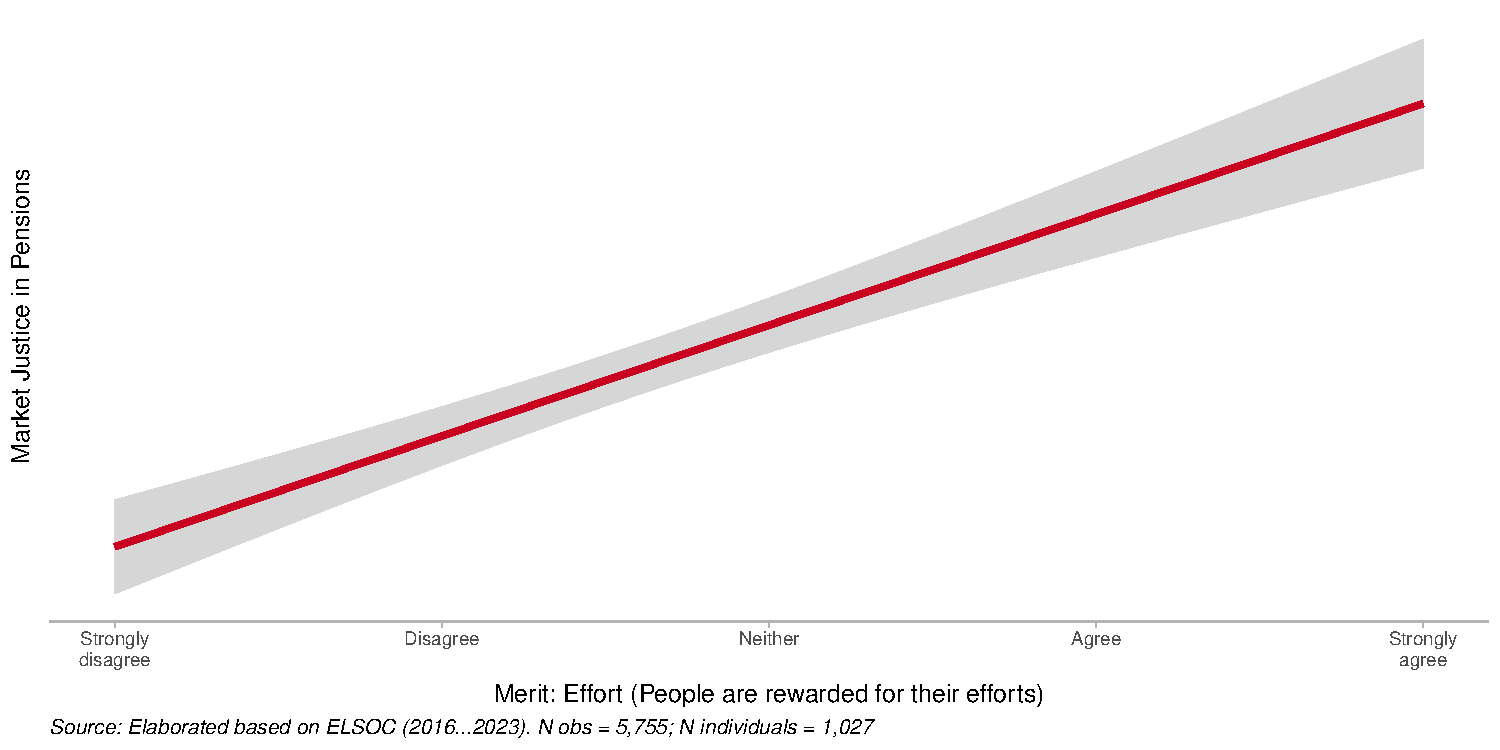
\includegraphics[width=0.85\linewidth,height=\textheight,keepaspectratio]{paper_files/figure-pdf/fig-scatter-merit-1.pdf}

}

\end{figure}%

\begin{figure}[H]

\caption{\label{fig-scatter-talent}Bivariate relationship between merit
(talent) and market justice in pensions}

\centering{

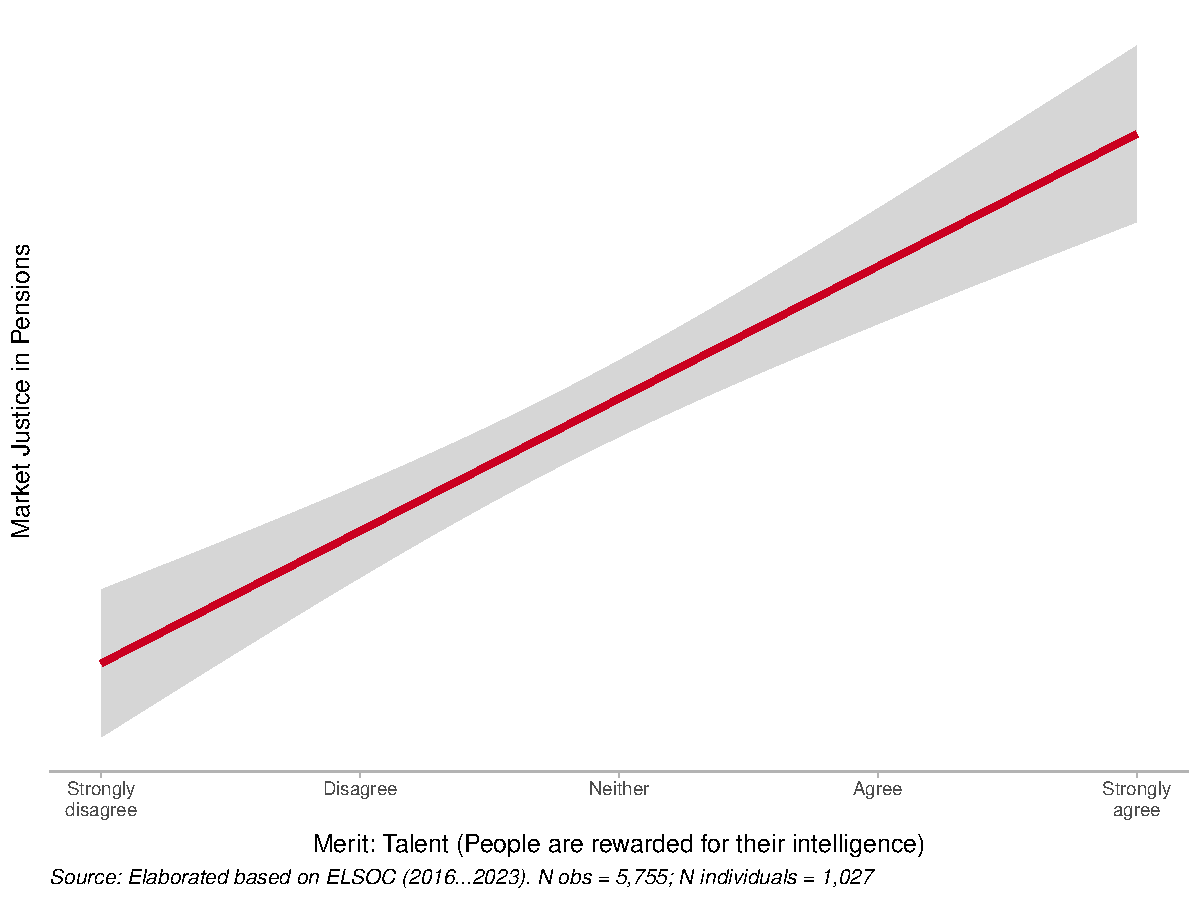
\includegraphics[width=0.85\linewidth,height=\textheight,keepaspectratio]{paper_files/figure-pdf/fig-scatter-talent-1.pdf}

}

\end{figure}%

Figure~\ref{fig-scatter-merit} and Figure~\ref{fig-scatter-talent}
present the bivariate relationships between meritocratic beliefs and
market justice preferences in pensions. Both figures reveal a clear
positive linear association: as individuals increasingly agree that
society rewards effort (Figure~\ref{fig-scatter-merit}) or talent
(Figure~\ref{fig-scatter-talent}), they are more likely to justify
inequalities in the pension system. The regression lines, accompanied by
their 95\% confidence intervals (shaded areas), demonstrate
statistically significant relationships across the full range of both
independent variables, with the confidence bands remaining relatively
narrow throughout, indicating robust and precise estimates.

\begin{figure}[H]

\caption{\label{fig-scatter-corr}Correlation matrix between meritocratic
beliefs and market justice}

\centering{


\includegraphics[width=0.85\linewidth,height=\textheight,keepaspectratio]{paper_files/figure-pdf/fig-scatter-corr-1.pdf}

}

\end{figure}%

The strength of these bivariate associations is further quantified in
Figure~\ref{fig-scatter-corr}, which presents the correlation matrix
between the three key variables. The correlation between Merit: Effort
and Market Justice in Pensions is \(r\) = 0.10 (p \textless{} 0.001),
while the correlation between Merit: Talent and Market Justice in
Pensions is slightly weaker at \(r\) = 0.08 (p \textless{} 0.001).
Although both correlations are modest in magnitude, they are highly
statistically significant given the large sample size (N obs = 5,755; N
individuals = 1,027). Notably, the two meritocratic belief
dimensions---effort and talent---show a strong positive correlation with
each other (\(r\) = 0.68, p \textless{} 0.001), suggesting they tap into
a common underlying meritocratic worldview, while maintaining sufficient
independence to be examined as distinct constructs.

These bivariate patterns provide initial empirical support for the
theoretical expectation that meritocratic beliefs are associated with
greater acceptance of market-based pension inequalities. However, the
relatively modest effect sizes indicate that the relationship is not
deterministic and that other factors---such as social class position,
political ideology, and individual experiences with the pension
system---likely play important moderating or confounding roles. The
subsequent multivariate analyses will test whether these bivariate
associations hold when controlling for relevant covariates and will
explore potential interaction effects between meritocratic beliefs and
social class, as hypothesized in our theoretical framework.

\subsection{Multilevel models}\label{multilevel-models}

Table~\ref{tbl-modelos} reports estimates from the cumulative multilevel
models of support for pension market justice, distinguishing effects
operating between individuals and within individuals over time. The
intraclass correlation coefficient
(\citeproc{ref-hox_multilevel_2017}{\textbf{hox\_multilevel\_2017?}})
from the null model (see \hyperref[anexo]{Supplementary Material}),
which partitions the total variance in the outcome, is 0.24. This
implies that about 24\% of the variance lies between individuals, while
the remaining 76\% reflects within-person change across survey waves.

Model 1, which adds survey-wave indicators to capture temporal shifts in
the outcome, shows a decline in 2017 (\(\beta\) = -0.337, \(p\)
\textless{} 0.001) relative to 2016. By contrast, the 2022 and 2023
waves exhibit significant increases in market justice preferences for
pension (\(\beta\) = 0.879, \(p\) \textless{} 0.001; \(\beta\) = 0.854,
\(p\) \textless{} 0.001), indicating a nonlinear pattern over time. To
account for this trajectory, Model 2 specifies time (survey wave) as a
continuous predictor and includes a quadratic term to capture the
curvature suggested by Model 1. The negative linear coefficient
indicates an overall downward trend in market-based access to old-age
pension benefits, whereas the positive quadratic term signals a
subsequent upturn in the final measurement points.

\begin{table}

\caption{\label{tbl-modelos}Cumulative link longitudinal multilevel
models for pension market justice preferences}

\centering{

\caption{}
\begin{center}
\scalebox{0.8}{
\begin{tabular}{l c c c c c c}
\hline
 & Model 1 & Model 2 & Model 3 & Model 4 & Model 5 & Model 6 \\
\hline
Wave (Ref.= 2016)                            &                &               &               &               &               &               \\
                                             &                &               &               &               &               &               \\
\quad Wave 2017                              & $-0.337^{***}$ &               &               &               &               &               \\
                                             & $(0.079)$      &               &               &               &               &               \\
\quad Wave 2018                              & $-0.013$       &               &               &               &               &               \\
                                             & $(0.078)$      &               &               &               &               &               \\
\quad Wave 2019                              & $0.086$        &               &               &               &               &               \\
                                             & $(0.077)$      &               &               &               &               &               \\
\quad Wave 2022                              & $0.879^{***}$  &               &               &               &               &               \\
                                             & $(0.078)$      &               &               &               &               &               \\
\quad Wave 2023                              & $0.854^{***}$  &               &               &               &               &               \\
                                             & $(0.077)$      &               &               &               &               &               \\
Wave                                         &                & $-0.182^{**}$ & $-0.179^{**}$ & $-0.187^{**}$ & $-0.190^{**}$ & $-0.192^{**}$ \\
                                             &                & $(0.064)$     & $(0.064)$     & $(0.064)$     & $(0.064)$     & $(0.064)$     \\
Wave$^2$                                     &                & $0.059^{***}$ & $0.058^{***}$ & $0.060^{***}$ & $0.060^{***}$ & $0.060^{***}$ \\
                                             &                & $(0.009)$     & $(0.009)$     & $(0.009)$     & $(0.009)$     & $(0.009)$     \\
Social class (Ref.= Working class (V+VI+VII) &                &               &               &               &               &               \\
                                             &                &               &               &               &               &               \\
\quad Intermediate class (III+IV)            &                &               & $0.096$       & $0.101$       & $0.147$       & $0.185$       \\
                                             &                &               & $(0.120)$     & $(0.121)$     & $(0.118)$     & $(0.117)$     \\
\quad Service class (I+II)                   &                &               & $0.169$       & $0.169$       & $0.158$       & $0.017$       \\
                                             &                &               & $(0.108)$     & $(0.108)$     & $(0.106)$     & $(0.109)$     \\
\quad Retired or pensioner                   &                &               & $0.103$       & $0.096$       & $0.030$       & $0.110$       \\
                                             &                &               & $(0.117)$     & $(0.117)$     & $(0.115)$     & $(0.127)$     \\
\quad Unemployed                             &                &               & $0.101$       & $0.105$       & $0.147$       & $0.119$       \\
                                             &                &               & $(0.158)$     & $(0.158)$     & $(0.155)$     & $(0.152)$     \\
\quad Performs unpaid tasks                  &                &               & $-0.199$      & $-0.198$      & $-0.208$      & $0.029$       \\
                                             &                &               & $(0.110)$     & $(0.111)$     & $(0.109)$     & $(0.113)$     \\
Merit: Effort (WE)                           &                &               &               & $0.114^{**}$  & $0.117^{***}$ & $0.115^{**}$  \\
                                             &                &               &               & $(0.035)$     & $(0.035)$     & $(0.035)$     \\
Merit: Talent (WE)                           &                &               &               & $0.066$       & $0.066$       & $0.067$       \\
                                             &                &               &               & $(0.034)$     & $(0.034)$     & $(0.034)$     \\
Merit: Effort (BE)                           &                &               &               &               & $0.391^{***}$ & $0.387^{***}$ \\
                                             &                &               &               &               & $(0.097)$     & $(0.093)$     \\
Merit: Talent (BE)                           &                &               &               &               & $0.079$       & $0.028$       \\
                                             &                &               &               &               & $(0.097)$     & $(0.094)$     \\
\hline
Controls                                     & No             & No            & No            & No            & No            & Yes           \\
BIC                                          & $19107.264$    & $19166.031$   & $19199.863$   & $19182.632$   & $19144.360$   & $19097.183$   \\
Numb. obs.                                   & $7522$         & $7522$        & $7522$        & $7522$        & $7522$        & $7522$        \\
Num. groups: individuals                     & $1317$         & $1317$        & $1317$        & $1317$        & $1317$        & $1317$        \\
Var: individuals (Intercept)                 & $1.151$        & $1.334$       & $1.302$       & $1.288$       & $1.146$       & $1.014$       \\
Var: individuals, wave                       & $$             & $0.018$       & $0.018$       & $0.015$       & $0.015$       & $0.016$       \\
\hline
\multicolumn{7}{l}{\scriptsize{Note: Cells contain regression coefficients with standard errors in parentheses. $^{***}p<0.001$; $^{**}p<0.01$; $^{*}p<0.05$.}}
\end{tabular}
}
\label{table:coefficients}
\end{center}

}

\end{table}%

Model 3 adds between-group effects (BE) for social class, capturing
differences in average support for pension market justice across class
locations. Overall, the estimates provide no evidence of systematic
class differences in the support for market-based access to old-age
pension benefits. Using the working class as the reference group, those
in the intermediate class (\(\beta\) = 0.10, \(p\) \textgreater{} 0.05),
the service class (\(\beta\) = 0.17, \(p\) \textgreater{} 0.05),
retirees (\(\beta\) = 0.10, \(p\) \textgreater{} 0.05), and the
unemployed (\(\beta\) = 0.10, \(p\) \textgreater{} 0.05) exhibit
positive coefficients, but none reach conventional levels of statistical
significance. Likewise, individuals performing unpaid work (e.g.,
domestic or care work) show a negative coefficient relative to the
working class, which is not statistically significant (\(\beta\) =
-0.20, \(p\) \textgreater{} 0.05). Taken together, these results suggest
that neither class position nor being outside the labour force is
clearly associated with differences in preferences for pension market
justice at the between-individual level.

Models 4 and 5 extend the analysis by incorporating the within-person
(WE) and between-person (BE) components of the meritocratic variables.
Model 4 examines how changes in individuals' meritocratic perceptions
over time relate to their views on pension market justice. The estimates
show that the within-effect of perceiving that effort is rewarded is
positive and highly significant (\(p\) \textless{} 0.001). Holding all
other predictors constant, a one-point increase in effort-based
meritocratic perceptions for the same respondent between waves is
associated with a 0.11-point increase in the support for market-based
access to old-age pension benefits. Model 5, which captures
between-person differences, points in the same direction. On average,
respondents who see their society as more effort-meritocratic display
stronger market-oriented views on pensions, with a 0.39-point higher
score on the outcome, a statistically significant association. By
contrast, the corresponding indicators for the belief that intelligence
and ability are rewarded show no statistically significant association
with the support for market-based access to old-age pension benefits at
either the within (\(\beta\) = 0.07, \(p\) \textgreater{} 0.05)- or
between-person level (\(\beta\) = 0.08, \(p\) \textgreater{} 0.05).

Model 6 introduces the control variables. The within- and
between-effects of the main predictors remain stable in both sign and
significance, indicating that the associations are robust (see
\hyperref[anexo]{Supplementary Material} for the effects of the control
variables).

\begin{table}

\caption{\label{tbl-interactions1}Interactions for social class,
meritocracy, and pension market justice preferences}

\centering{

\caption{}
\begin{center}
\scalebox{0.8}{
\begin{tabular}{l c c c c}
\hline
 & Model 7 & Model 8 & Model 9 & Model 10 \\
\hline
Social class (Ref.= Working class (V+VI+VII)                    &               &               &               &               \\
                                                                &               &               &               &               \\
\quad Intermediate class (III+IV)                               & $0.249^{*}$   & $0.249^{*}$   & $-0.741$      & $-0.833$      \\
                                                                & $(0.119)$     & $(0.120)$     & $(0.522)$     & $(0.526)$     \\
\quad Service class (I+II)                                      & $0.210^{*}$   & $0.212^{*}$   & $-0.207$      & $-0.415$      \\
                                                                & $(0.105)$     & $(0.106)$     & $(0.462)$     & $(0.496)$     \\
\quad Retired or pensioner                                      & $0.197$       & $0.199$       & $-0.416$      & $-0.124$      \\
                                                                & $(0.129)$     & $(0.129)$     & $(0.508)$     & $(0.539)$     \\
\quad Unemployed                                                & $0.173$       & $0.178$       & $-0.219$      & $-0.166$      \\
                                                                & $(0.155)$     & $(0.156)$     & $(0.642)$     & $(0.713)$     \\
\quad Performs unpaid tasks                                     & $0.064$       & $0.062$       & $0.305$       & $0.493$       \\
                                                                & $(0.115)$     & $(0.116)$     & $(0.446)$     & $(0.494)$     \\
Merit: Effort (WE)                                              & $0.074$       & $0.123^{***}$ & $0.116^{***}$ & $0.116^{***}$ \\
                                                                & $(0.059)$     & $(0.036)$     & $(0.035)$     & $(0.035)$     \\
Merit: Talent (WE)                                              & $0.066$       & $-0.024$      & $0.067$       & $0.067$       \\
                                                                & $(0.035)$     & $(0.057)$     & $(0.034)$     & $(0.034)$     \\
Merit: Effort (BE)                                              & $0.385^{***}$ & $0.409^{***}$ & $0.304^{*}$   & $0.405^{***}$ \\
                                                                & $(0.096)$     & $(0.096)$     & $(0.128)$     & $(0.094)$     \\
Merit: Talent (BE)                                              & $0.009$       & $-0.006$      & $0.000$       & $-0.089$      \\
                                                                & $(0.097)$     & $(0.097)$     & $(0.095)$     & $(0.130)$     \\
Social class (Ref.= Working class (V+VI+VII) x Meritocracy (WE) &               &               &               &               \\
                                                                &               &               &               &               \\
\quad Intermediate class (III+IV) x Merit: Effort (WE)          & $0.109$       &               &               &               \\
                                                                & $(0.100)$     &               &               &               \\
\quad Service class (I+II) x Merit: Effort (WE)                 & $0.080$       &               &               &               \\
                                                                & $(0.089)$     &               &               &               \\
\quad Retired or pensioner x Merit: Effort (WE)                 & $0.020$       &               &               &               \\
                                                                & $(0.091)$     &               &               &               \\
\quad Unemployed x Merit: Effort (WE)                           & $0.087$       &               &               &               \\
                                                                & $(0.134)$     &               &               &               \\
\quad Performs unpaid tasks x Merit: Effort (WE)                & $0.033$       &               &               &               \\
                                                                & $(0.092)$     &               &               &               \\
\quad Intermediate class (III+IV) x Merit: Talent (WE)          &               & $0.171$       &               &               \\
                                                                &               & $(0.099)$     &               &               \\
\quad Service class (I+II) x Merit: Talent (WE)                 &               & $0.091$       &               &               \\
                                                                &               & $(0.089)$     &               &               \\
\quad Retired or pensioner x Merit: Talent (WE)                 &               & $0.050$       &               &               \\
                                                                &               & $(0.091)$     &               &               \\
\quad Unemployed x Merit: Talent (WE)                           &               & $0.257^{*}$   &               &               \\
                                                                &               & $(0.131)$     &               &               \\
\quad Performs unpaid tasks x Merit: Talent (WE)                &               & $0.174$       &               &               \\
                                                                &               & $(0.092)$     &               &               \\
Social class (Ref.= Working class (V+VI+VII) x Meritocracy (BE) &               &               &               &               \\
                                                                &               &               &               &               \\
\quad Intermediate class (III+IV) x Merit: Effort (BE)          &               &               & $0.390$       &               \\
                                                                &               &               & $(0.201)$     &               \\
\quad Service class (I+II) x Merit: Effort (BE)                 &               &               & $0.157$       &               \\
                                                                &               &               & $(0.172)$     &               \\
\quad Retired or pensioner x Merit: Effort (BE)                 &               &               & $0.225$       &               \\
                                                                &               &               & $(0.182)$     &               \\
\quad Unemployed x Merit: Effort (BE)                           &               &               & $0.153$       &               \\
                                                                &               &               & $(0.248)$     &               \\
\quad Performs unpaid tasks x Merit: Effort (BE)                &               &               & $-0.095$      &               \\
                                                                &               &               & $(0.167)$     &               \\
\quad Intermediate class (III+IV) x Merit: Talent (BE)          &               &               &               & $0.401^{*}$   \\
                                                                &               &               &               & $(0.191)$     \\
\quad Service class (I+II) x Merit: Talent (BE)                 &               &               &               & $0.222$       \\
                                                                &               &               &               & $(0.174)$     \\
\quad Retired or pensioner x Merit: Talent (BE)                 &               &               &               & $0.111$       \\
                                                                &               &               &               & $(0.182)$     \\
\quad Unemployed x Merit: Talent (BE)                           &               &               &               & $0.123$       \\
                                                                &               &               &               & $(0.257)$     \\
\quad Performs unpaid tasks x Merit: Talent (BE)                &               &               &               & $-0.157$      \\
                                                                &               &               &               & $(0.174)$     \\
\hline
Controls                                                        & Yes           & Yes           & Yes           & Yes           \\
BIC                                                             & $19167.451$   & $19152.429$   & $19152.225$   & $19150.549$   \\
Numb. obs.                                                      & $7522$        & $7522$        & $7522$        & $7522$        \\
Num. groups: individuals                                        & $1317$        & $1317$        & $1317$        & $1317$        \\
Var: individuals (Intercept)                                    & $1.112$       & $1.116$       & $1.073$       & $1.063$       \\
Var: individuals, wave                                          & $0.014$       & $0.013$       & $0.015$       & $0.015$       \\
Var: individuals, merit effort cwc                              & $0.112$       & $$            & $$            & $$            \\
Var: individuals, merit talent cwc                              & $$            & $0.142$       & $$            & $$            \\
\hline
\multicolumn{5}{l}{\scriptsize{Note: Cells contain regression coefficients with standard errors in parentheses. $^{***}p<0.001$; $^{**}p<0.01$; $^{*}p<0.05$. CWC = centered within group.}}
\end{tabular}
}
\label{table:coefficients}
\end{center}

}

\end{table}%

To examine whether meritocratic perceptions condition class differences
in market justice preferences in pensions, Table~\ref{tbl-interactions1}
reports four interaction models that combine between-person social class
with the within- and between-person components of meritocratic
perceptions. Model 7 includes interactions between class and
within-person effort-based meritocracy; Model 8 does the same for
within-person talent-based meritocracy; Model 9 interacts class with
between-person effort-based meritocracy; and Model 10 with
between-person talent-based meritocracy. Overall, the interaction terms
are small and mostly non-significant, and model fit improves only
marginally relative to the baseline specifications, suggesting that the
link between meritocratic perceptions and market justice preferences in
pensions is broadly similar across social classes.

Two interaction effects stand out as exceptions to this general pattern.
In Model 8, the interaction between unemployment and within-person
talent-based meritocracy is positive and statistically significant
(\(\beta\) = 0.26, \(p\) \textless{} 0.05), indicating that, among
unemployed respondents, increases over time in the perception that
intelligence and ability are rewarded are more strongly associated with
stronger support for market-based access to old-age pension benefits
than among working-class respondents. In Model 10, the interaction
between an intermediate-class position and between-person talent-based
meritocracy is also positive and significant (\(\beta\) = 0.40, \(p\)
\textless{} 0.05), implying that, within the intermediate class,
individuals who more strongly believe that talent is rewarded display a
steeper increase in market-oriented views on pensions than their
working-class counterparts. Taken together, the evidence points to a
largely homogeneous association between meritocracy and justice, with
only limited moderation, concentrated in the talent dimension and in
specific non-core classes.

\section{Discussion}\label{discussion}

Survey evidence from 2016 to 2023 points to marked ambivalence among
Chileans in their evaluation of market-based pension justice. In each
wave, clear majorities reject the notion that it is fair for
higher-income individuals to receive better pensions than lower-income
individuals. At the same time, a small but expanding segment of
respondents endorses this income-based principle, with the steepest
growth occurring between 2018 and 2023. Market allocation of pension
benefits thus remains a minority preference, yet one that has become
more prevalent over time, in line with longitudinal evidence of rising
support for income-based access to welfare services in Chile
(\citeproc{ref-castillo_perceptions_2025}{Juan Carlos Castillo et al.,
2025}). These attitudes are formed within an institutional architecture
of mandatory, privately managed, defined-contribution accounts that
closely tie old-age income to labor earnings, contribution stability,
and market performance
(\citeproc{ref-madero-cabib_private_2019}{Madero-Cabib et al., 2019};
\citeproc{ref-solimano_rise_2021}{Solimano, 2021}), and that
symbolically recast pensions from solidarity-based social rights into
individual financial assets. In this respect, Chile mirrors broader
findings that income-based access to welfare is more strongly endorsed
in liberal, marketised regimes (\citeproc{ref-lindh_public_2015}{Lindh,
2015}). Taken together, these patterns suggest that support for pension
commodification, although contested and far from hegemonic, constitutes
a salient orientation that raises the question of which social
trajectories and belief structures sustain it.

\section{Conclusion}\label{conclusion}

\section{References}\label{references}

\phantomsection\label{refs}
\begin{CSLReferences}{1}{0}
\bibitem[\citeproctext]{ref-arenas_sistemas_2019}
Arenas, A. (2019). \emph{{Los sistemas de pensiones en la encrucijada:
desafíos para la sostenibilidad en América Latina}}. Santiago: Naciones
Unidas, CEPAL.

\bibitem[\citeproctext]{ref-arrizabalomontoro_debate_2019}
Arrizabalo Montoro, X., Del Rosal, M., \& Javier Murillo Arroyo, F.
(2019). The {Debate} on {Pension Systems}: {The Paradigmatic Cases} of
{Chile} and {Spain}. \emph{The American Journal of Economics and
Sociology}, \emph{78}(1), 195--223.
\url{https://doi.org/10.1111/ajes.12262}

\bibitem[\citeproctext]{ref-barone_rise_2022}
Barone, C., Hertel, F. R., \& Smallenbroek, O. (2022). The rise of
income and the demise of class and social status? {A} systematic review
of measures of socio-economic position in stratification research.
\emph{Research in Social Stratification and Mobility}, \emph{78},
100678. \url{https://doi.org/10.1016/j.rssm.2022.100678}

\bibitem[\citeproctext]{ref-barozet_measurement_2021}
Barozet, E., Boado, M., \& Marqués-Perales, I. (2021). The {Measurement}
of {Social Stratification}: {Comparative Perspectives Between Europe}
and {Latin America}. In P. López-Roldán \& S. Fachelli (Eds.),
\emph{Towards a {Comparative Analysis} of {Social Inequalities} between
{Europe} and {Latin America}} (pp. 171--202). Cham: Springer
International Publishing.
\url{https://doi.org/10.1007/978-3-030-48442-2_6}

\bibitem[\citeproctext]{ref-beland_varieties_2019}
Béland, D., \& Schlager, E. (2019). Varieties of {Policy Feedback
Research}: {Looking Backward}, {Moving Forward}. \emph{Policy Studies
Journal}, \emph{47}(2), 184--205.
\url{https://doi.org/10.1111/psj.12340}

\bibitem[\citeproctext]{ref-bell_fixed_2019}
Bell, A., Fairbrother, M., \& Jones, K. (2019). Fixed and random effects
models: Making an informed choice. \emph{Quality \& Quantity},
\emph{53}(2), 1051--1074.
\url{https://doi.org/10.1007/s11135-018-0802-x}

\bibitem[\citeproctext]{ref-bell_explaining_2015}
Bell, A., \& Jones, K. (2015). Explaining {Fixed Effects}: {Random
Effects Modeling} of {Time-Series Cross-Sectional} and {Panel Data}.
\emph{Political Science Research and Methods}, \emph{3}(1), 133--153.
\url{https://doi.org/10.1017/psrm.2014.7}

\bibitem[\citeproctext]{ref-boccardo_30_2020}
Boccardo, G. (2020). \emph{30 años de privatizaciones en {Chile}: {Lo}
que la pandemia reveló}. Nodo XXI.

\bibitem[\citeproctext]{ref-borzutzky_chiles_2016}
Borzutzky, S., \& Hyde, M. (2016). Chile's private pension system at 35:
Impact and lessons. \emph{Journal of International and Comparative
Social Policy}, \emph{32}(1), 57--73.
\url{https://doi.org/10.1080/21699763.2016.1148623}

\bibitem[\citeproctext]{ref-breen_foundations_2005}
Breen, R. (2005). Foundations of a neo-{Weberian} class analysis. In E.
O. Wright (Ed.), \emph{Approaches to {Class Analysis}} (1st ed., pp.
31--50). Cambridge University Press.
\url{https://doi.org/10.1017/CBO9780511488900.003}

\bibitem[\citeproctext]{ref-breznau_institutional_2023}
Breznau, N. (2023). Institutional trajectories of the welfare state:
Returns from social policy inception to modern public opinion. In F.
Roosma \& T. Laenen (Eds.), \emph{A {Research Agenda} for {Public
Attitudes} to {Welfare}} (pp. 185--205). Edward Elgar Publishing.
\url{https://doi.org/10.4337/9781800887411.00015}

\bibitem[\citeproctext]{ref-bril-mascarenhas_how_2019}
Bril-Mascarenhas, T., \& Maillet, A. (2019). How to {Build} and {Wield
Business Power}: {The Political Economy} of {Pension Regulation} in
{Chile}, 1990--2018. \emph{Latin American Politics and Society},
\emph{61}(1), 101--125. \url{https://doi.org/10.1017/lap.2018.61}

\bibitem[\citeproctext]{ref-busemeyer_education_2013}
Busemeyer, M. R. (2013). Education {Funding} and {Individual
Preferences} for {Redistribution}. \emph{European Sociological Review},
\emph{29}(6), 1122--1133. \url{https://doi.org/10.1093/esr/jcs085}

\bibitem[\citeproctext]{ref-busemeyer_welfare_2020}
Busemeyer, M. R., \& Iversen, T. (2020). The {Welfare State} with
{Private Alternatives}: {The Transformation} of {Popular Support} for
{Social Insurance}. \emph{The Journal of Politics}, \emph{82}(2),
671--686. \url{https://doi.org/10.1086/706980}

\bibitem[\citeproctext]{ref-cabib_avoiding_2025}
Cabib, I. (2025). \emph{Avoiding {Retirement} in {Chile}: {Extending
Working Lives} in an {Uncertain} and {Precarious Context}}. London:
Routledge.

\bibitem[\citeproctext]{ref-canalesceron_sujeto_2021}
Canales Cerón, M., Orellana Calderón, V. S., \& Guajardo Mañán, F.
(2021). Sujeto y cotidiano en la era neoliberal: El caso de la educación
chilena. \emph{Revista Mexicana de Ciencias Políticas y Sociales},
\emph{67}(244).
\url{https://doi.org/10.22201/fcpys.2448492xe.2022.244.70386}

\bibitem[\citeproctext]{ref-castillo_multidimensional_2023}
Castillo, Juan Carlos, Iturra, J., Maldonado, L., Atria, J., \& Meneses,
F. (2023). A {Multidimensional Approach} for {Measuring Meritocratic
Beliefs}: {Advantages}, {Limitations} and {Alternatives} to the {ISSP
Social Inequality Survey}. \emph{International Journal of Sociology},
\emph{53}(6), 448--472.
\url{https://doi.org/10.1080/00207659.2023.2274712}

\bibitem[\citeproctext]{ref-castillo_perceptions_2025}
Castillo, Juan Carlos, Laffert, A., Carrasco, K., \& Iturra-Sanhueza, J.
(2025). Perceptions of inequality and meritocracy: Their interplay in
shaping preferences for market justice in {Chile} (2016--2023).
\emph{Frontiers in Sociology}, \emph{10}, 1634219.
\url{https://doi.org/10.3389/fsoc.2025.1634219}

\bibitem[\citeproctext]{ref-castillo_socialization_2024}
Castillo, Juan Carlos, Salgado, M., Carrasco, K., \& Laffert, A. (2024).
The {Socialization} of {Meritocracy} and {Market Justice Preferences} at
{School}. \emph{Societies}, \emph{14}(11), 214.
\url{https://doi.org/10.3390/soc14110214}

\bibitem[\citeproctext]{ref-castillo_deserving_2019}
Castillo, Juan-Carlos, Olivos, F., \& Azar, A. (2019). Deserving a {Just
Pension}: {A Factorial Survey Approach}*. \emph{Social Science
Quarterly}, \emph{100}(1), 359--378.
\url{https://doi.org/10.1111/ssqu.12539}

\bibitem[\citeproctext]{ref-chancel_world_2022}
Chancel, L., Piketty, T., Saez, E., \& Zucman, G. (2022). \emph{{WORLD
INEQUALITY REPORT} 2022} (p. 230).

\bibitem[\citeproctext]{ref-dodson_economic_2017}
Dodson, K. (2017). Economic {Change} and {Class Conflict} over {Tax
Attitudes}: {Evidence} from {Nine Advanced Capitalist Democracies}.
\emph{Social Forces}, \emph{95}(4), 1509--1538.
\url{https://doi.org/10.1093/sf/sox027}

\bibitem[\citeproctext]{ref-edlund_democratic_2015}
Edlund, J., \& Lindh, A. (2015). The democratic class struggle
revisited: {The} welfare state, social cohesion and political conflict.
\emph{Acta Sociologica}, \emph{58}(4), 311--328.
\url{https://doi.org/10.1177/0001699315610176}

\bibitem[\citeproctext]{ref-erikson_constant_1992}
Erikson, R., \& Goldthorpe, J. (1992a). \emph{The constant flux: A study
of class mobility in industrial societies}. Oxford: Clarendon Pr.

\bibitem[\citeproctext]{ref-erikson_casmin_1992}
Erikson, R., \& Goldthorpe, J. H. (1992b). The {CASMIN} project and the
{American} dream. \emph{European Sociological Review}, \emph{8}(3),
283--305. \url{https://doi.org/10.1093/oxfordjournals.esr.a036642}

\bibitem[\citeproctext]{ref-esping-andersen_three_1990}
Esping-Andersen, G. (1990). \emph{The {Three Worlds} of {Welfare
Capitalism}}. Cambridge: Polity Press.

\bibitem[\citeproctext]{ref-evans_assessing_2024}
Evans, C., \& Pienknagura, S. (2024). Assessing {Chile}\&rsquo;s
{Pension System}: {Challenges} and {Reform Options}. \emph{Economía},
\emph{23}(1). \url{https://doi.org/10.31389/eco.420}

\bibitem[\citeproctext]{ref-evans_conditional_2022}
Evans, G., Stubager, R., \& Langsæther, P. E. (2022). The conditional
politics of class identity: Class origins, identity and political
attitudes in comparative perspective. \emph{West European Politics},
\emph{45}(6), 1178--1205.
\url{https://doi.org/10.1080/01402382.2022.2039980}

\bibitem[\citeproctext]{ref-ferre_welfare_2023}
Ferre, J. C. (2023). Welfare regimes in twenty-first-century {Latin
America}. \emph{Journal of International and Comparative Social Policy},
\emph{39}(2), 101--127. \url{https://doi.org/10.1017/ics.2023.16}

\bibitem[\citeproctext]{ref-flores_top_2020}
Flores, I., Sanhueza, C., Atria, J., \& Mayer, R. (2020). Top {Incomes}
in {Chile}: {A Historical Perspective} on {Income Inequality},
1964--2017. \emph{Review of Income and Wealth}, \emph{66}(4), 850--874.
\url{https://doi.org/10.1111/roiw.12441}

\bibitem[\citeproctext]{ref-galvez_pensiones_2024}
Gálvez, R., Kremerman, M., \& Palacios, V. R. (2024). {Pensiones bajo el
mínimo: Los montos de las pensiones que paga el sistema de
capitalización individual en Chile}. \emph{Fundación Sol}.

\bibitem[\citeproctext]{ref-gingrich_making_2011}
Gingrich, J. R. (2011). \emph{Making {Markets} in the {Welfare State}:
{The Politics} of {Varying Market Reforms}} (1st ed.). Cambridge
University Press. \url{https://doi.org/10.1017/CBO9780511791529}

\bibitem[\citeproctext]{ref-harrs_fairness_2025}
Harrs, S., \& Sterba, M.-B. (2025). \emph{Fairness and {Support} for
{Redistribution}: {The Role} of {Preferences} and {Beliefs}}. University
of Konstanz. \url{https://doi.org/10.48787/KOPS/352-2-1795HQRPSTDTX1}

\bibitem[\citeproctext]{ref-huber_political_2000}
Huber, E., \& Stephens, J. D. (2000). The political economy of pension
reform: {Latin America} in comparative perspective. \emph{Occasional
Paper}, (7).

\bibitem[\citeproctext]{ref-hyde_chiles_2015}
Hyde, M., \& Borzutzky, S. (2015). Chile's {``{Neoliberal}''}
{Retirement System}? {Concentration}, {Competition}, and {Economic
Predation} in {``{Private}''} {Pensions}: {Chile}'s {``{Neoliberal}''}
{Retirement System}? \emph{Poverty \& Public Policy}, \emph{7}(2),
123--157. \url{https://doi.org/10.1002/pop4.98}

\bibitem[\citeproctext]{ref-immergut_it_2020}
Immergut, E. M., \& Schneider, S. M. (2020). Is it unfair for the
affluent to be able to purchase {``better''} healthcare? {Existential}
standards and institutional norms in healthcare attitudes across 28
countries. \emph{Social Science \& Medicine}, \emph{267}, 113146.
\url{https://doi.org/10.1016/j.socscimed.2020.113146}

\bibitem[\citeproctext]{ref-iturra-sanhueza_classbased_2025}
Iturra-Sanhueza, J. (2025). Class-based network segregation, economic
inequality, and redistributive preferences across societies.
\emph{European Sociological Review}, jcaf048.
\url{https://doi.org/10.1093/esr/jcaf048}

\bibitem[\citeproctext]{ref-jaime-castillo_public_2013}
Jaime-Castillo, A. M. (2013). Public opinion and the reform of the
pension systems in {Europe}: The influence of solidarity principles.
\emph{Journal of European Social Policy}, \emph{23}(4), 390--405.
\url{https://doi.org/10.1177/0958928713507468}

\bibitem[\citeproctext]{ref-kerner_pension_2020}
Kerner, A. (2020). Pension {Returns} and {Popular Support} for
{Neoliberalism} in {Post-Pension Reform Latin America}. \emph{British
Journal of Political Science}, \emph{50}(2), 585--620.
\url{https://doi.org/10.1017/S0007123417000710}

\bibitem[\citeproctext]{ref-kluegel_beliefs_1981}
Kluegel, J. R., \& Smith, E. R. (1981). Beliefs about {Stratification}.
\emph{Annual Review of Sociology}, \emph{7}(Volume 7, 1981), 29--56.
\url{https://doi.org/10.1146/annurev.so.07.080181.000333}

\bibitem[\citeproctext]{ref-kluegel_legitimation_1999}
Kluegel, J., Mason, D., \& Wegener, B. (1999). The {Legitimation} of
{Capitalism} in the {Postcommunist Transition}: {Public Opinion} about
{Market Justice}, 1991-1996. \emph{European Sociological Review},
\emph{15}(3), 33. Retrieved from
\url{https://www.jstor.org/stable/522731}

\bibitem[\citeproctext]{ref-koos_moral_2019}
Koos, S., \& Sachweh, P. (2019). The moral economies of market
societies: Popular attitudes towards market competition, redistribution
and reciprocity in comparative perspective. \emph{Socio-Economic
Review}, \emph{17}(4), 793--821.
\url{https://doi.org/10.1093/ser/mwx045}

\bibitem[\citeproctext]{ref-korpi_power_2006}
Korpi, W. (2006). Power {Resources} and {Employer-Centered Approaches}
in {Explanations} of {Welfare States} and {Varieties} of {Capitalism}:
{Protagonists}, {Consenters}, and {Antagonists}. \emph{World Politics},
\emph{58}(2), 167--206. \url{https://doi.org/10.1353/wp.2006.0026}

\bibitem[\citeproctext]{ref-korpi_democratic_2018}
Korpi, W. (2018). \emph{The {Democratic Class Struggle}} (1st ed.).
Routledge. \url{https://doi.org/10.4324/9780429441714}

\bibitem[\citeproctext]{ref-korpi_new_2003}
Korpi, W., \& Palme, J. (2003). New {Politics} and {Class Politics} in
the {Context} of {Austerity} and {Globalization}: {Welfare State
Regress} in 18 {Countries}, 1975--95. \emph{American Political Science
Review}, \emph{97}(03). \url{https://doi.org/10.1017/S0003055403000789}

\bibitem[\citeproctext]{ref-lane_market_1986}
Lane, R. E. (1986). Market {Justice}, {Political Justice}.
\emph{American Political Science Review}, \emph{80}(2), 383--402.
\url{https://doi.org/10.2307/1958264}

\bibitem[\citeproctext]{ref-langsaether_more_2020}
Langsæther, P. E., \& Evans, G. (2020). More than self-interest: {Why}
different classes have different attitudes to income inequality.
\emph{The British Journal of Sociology}, \emph{71}(4), 594--607.
\url{https://doi.org/10.1111/1468-4446.12747}

\bibitem[\citeproctext]{ref-langsaether_explaining_2022}
Langsæther, P. E., Evans, G., \& O'Grady, T. (2022). Explaining the
{Relationship Between Class Position} and {Political Preferences}: {A
Long-Term Panel Analysis} of {Intra-Generational Class Mobility}.
\emph{British Journal of Political Science}, \emph{52}(2), 958--967.
\url{https://doi.org/10.1017/S0007123420000599}

\bibitem[\citeproctext]{ref-lee_fairness_2024}
Lee, J.-S., \& Stacey, M. (2024). Fairness perceptions of educational
inequality: The effects of self-interest and neoliberal orientations.
\emph{The Australian Educational Researcher}, \emph{51}(4), 1215--1237.
\url{https://doi.org/10.1007/s13384-023-00636-6}

\bibitem[\citeproctext]{ref-liebig_sociology_2016}
Liebig, S., \& Sauer, C. (2016). Sociology of {Justice}. In C. Sabbagh
\& M. Schmitt (Eds.), \emph{Handbook of {Social Justice Theory} and
{Research}} (pp. 37--59). New York: Springer.
\url{https://doi.org/10.1007/978-1-4939-3216-0_3}

\bibitem[\citeproctext]{ref-lindh_public_2015}
Lindh, A. (2015). Public {Opinion} against {Markets}? {Attitudes}
towards {Market Distribution} of {Social Services} -- {A Comparison} of
17 {Countries}. \emph{Social Policy \& Administration}, \emph{49}(7),
887--910. \url{https://doi.org/10.1111/spol.12105}

\bibitem[\citeproctext]{ref-lindh_it_2017}
Lindh, A. (2017). Is it {Just} that {People} with {Higher Incomes Can
Buy Better Education} and {Health Care}? \emph{57225}, \emph{17},
69--80.

\bibitem[\citeproctext]{ref-littler_meritocracy_2018}
Littler, J. (2018). \emph{Against meritocracy: Culture, power and myths
of mobility}. Abingdon, Oxon New York, NY: Routledge, an imprint of the
Taylor \& Francis group.

\bibitem[\citeproctext]{ref-llambias-wolff_political_2019}
Llambías-Wolff, J. (2019). The {Political Economy} of {Health Reforms}
in {Chile}: {A Case Study} of the {Privatization Process}. In D. Burke,
P. Godbole, \& A. Cash (Eds.), \emph{Hospital {Transformation}} (pp.
59--70). Cham: Springer International Publishing.
\url{https://doi.org/10.1007/978-3-030-15448-6_8}

\bibitem[\citeproctext]{ref-madariaga_three_2020}
Madariaga, A. (2020). The three pillars of neoliberalism: {Chile}'s
economic policy trajectory in comparative perspective.
\emph{Contemporary Politics}, \emph{26}(3), 308--329.
\url{https://doi.org/10.1080/13569775.2020.1735021}

\bibitem[\citeproctext]{ref-madero-cabib_private_2019}
Madero-Cabib, I., Biehl, A., Sehnbruch, K., Calvo, E., \& Bertranou, F.
(2019). Private {Pension Systems Built} on {Precarious Foundations}: {A
Cohort Study} of {Labor-Force Trajectories} in {Chile}. \emph{Research
on Aging}, \emph{41}(10), 961--987.
\url{https://doi.org/10.1177/0164027519874687}

\bibitem[\citeproctext]{ref-mau_inequality_2015}
Mau, S. (2015). \emph{Inequality, {Marketization} and the {Majority
Class}: {Why Did} the {European Middle Classes Accept Neo-Liberalism}?}
London: Palgrave Macmillan UK.

\bibitem[\citeproctext]{ref-mcnamee_meritocracy_2004}
McNamee, S., \& Miller, R. (2004). \emph{The meritocracy myth} (2004th
ed.). Lanham Md.: Rowman \& Littlefield.

\bibitem[\citeproctext]{ref-mijs_paradox_2019}
Mijs, J. J. B. (2019). The paradox of inequality: Income inequality and
belief in meritocracy go hand in hand. \emph{Socio-Economic Review}.
\url{https://doi.org/10.1093/ser/mwy051}

\bibitem[\citeproctext]{ref-mijs_paradox_2021}
Mijs, J. J. B. (2021). The paradox of inequality: Income inequality and
belief in meritocracy go hand in hand. \emph{Socio-Economic Review},
\emph{19}(1), 7--35. \url{https://doi.org/10.1093/ser/mwy051}

\bibitem[\citeproctext]{ref-pakulski_death_1997}
Pakulski, J., \& Waters, M. (1997). The {Death} of {Class}.
\emph{Capital \& Class}, \emph{21}(2), 192--193.
\url{https://doi.org/10.1177/030981689706200114}

\bibitem[\citeproctext]{ref-perezahumada_class_2024}
Pérez Ahumada, P. (2024). Class, union membership, and organizational
commitment: {A} multilevel analysis of 28 countries. \emph{Economic and
Industrial Democracy}, \emph{45}(1), 219--245.
\url{https://doi.org/10.1177/0143831X221148235}

\bibitem[\citeproctext]{ref-pierson_when_1993}
Pierson, P. (1993). When {Effect Becomes Cause}: {Policy Feedback} and
{Political Change}. \emph{World Politics}, \emph{45}(4), 595--628.
\url{https://doi.org/10.2307/2950710}

\bibitem[\citeproctext]{ref-piketty_capital_2014}
Piketty, T. (2014). \emph{Capital in the twenty-first century}. (A.
Goldhammer, Trans.). Cambridge Massachusetts: The Belknap Press of
Harvard University Press.

\bibitem[\citeproctext]{ref-pnud_desiguales_2017}
PNUD. (2017). \emph{Desiguales: {Origenes}, cambios y desafíos de la
brecha social en {Chile}}. Santiago de Chile: Uqbar Editores.

\bibitem[\citeproctext]{ref-reynolds_perceptions_2014}
Reynolds, J., \& Xian, H. (2014). Perceptions of meritocracy in the land
of opportunity. \emph{Research in Social Stratification and Mobility},
\emph{36}, 121--137. \url{https://doi.org/10.1016/j.rssm.2014.03.001}

\bibitem[\citeproctext]{ref-rosenzvaig-hernandez_unmaking_2024}
Rosenzvaig-Hernandez, M. (2024). Unmaking the market: Exploring the
{Chilean} challenges to de-privatise the educational system.
\emph{Globalisation, Societies and Education}, \emph{22}(5), 856--874.
\url{https://doi.org/10.1080/14767724.2022.2119123}

\bibitem[\citeproctext]{ref-rothstein_just_1998}
Rothstein, B. (1998). \emph{Just {Institutions Matter}: {The Moral} and
{Political Logic} of the {Universal Welfare State}} (1st ed.). Cambridge
University Press. \url{https://doi.org/10.1017/CBO9780511598449}

\bibitem[\citeproctext]{ref-rozasbugueno_entre_2019}
Rozas Bugueño, J., \& Maillet, A. (2019). Entre marchas, plebiscitos e
iniciativas de ley: Innovación en el repertorio de estrategias del
movimiento {No Más AFP} en {Chile} (2014-2018). \emph{Izquierdas}, (48),
1--21. \url{https://doi.org/10.4067/S0718-50492019000400001}

\bibitem[\citeproctext]{ref-singer_applied_2003}
Singer, J. D. (2003). \emph{Applied {Longitudinal Data Analysis}:
{Modeling Change} and {Event Occurrence}}. Cary: Oxford University
Press, Incorporated.

\bibitem[\citeproctext]{ref-solimano_rise_2021}
Solimano, A. (2021). \emph{The {Rise} and {Fall} of the {Privatized
Pension System} in {Chile}}. Anthem Press.

\bibitem[\citeproctext]{ref-subsecretariadeprevisionsocial_percepcion_2023}
Subsecretaría de Previsión Social. (2023). \emph{Percepción de la
ciudadanía del sistema de pensiones chileno}. Santiago.

\bibitem[\citeproctext]{ref-svallfors_moral_2006}
Svallfors, S. (2006). \emph{The moral economy of class}. Stanford
University Press.

\bibitem[\citeproctext]{ref-svallfors_political_2007}
Svallfors, S. (Ed.). (2007). \emph{The {Political Sociology} of the
{Welfare State}: {Institutions}, {Social Cleavages}, and {Orientations}}
(1st ed.). Stanford University Press.
\url{https://doi.org/10.2307/j.ctvr0qv0q}

\bibitem[\citeproctext]{ref-verbic_political_2019}
Verbič, M., \& Spruk, R. (2019). Political economy of pension reforms:
An empirical investigation. \emph{European Journal of Law and
Economics}, \emph{47}(2), 171--232.
\url{https://doi.org/10.1007/s10657-018-9606-7}

\bibitem[\citeproctext]{ref-wright_class_2000}
Wright, E. O. (2000). \emph{Class counts: Comparative studies in class
analysis} (Reprinted). Cambridge: Cambridge Univ. Press {[}u.a.{]}.

\bibitem[\citeproctext]{ref-young_rise_1975}
Young, M. D. (1975). \emph{The rise of the meritocracy: 1870 - 2033; an
essay on education and equality} (Repr). Harmondsworth: Penguin Books.

\end{CSLReferences}




\end{document}
